%\begin{savequote}[75mm]
%This is some random quote to start off the chapter.
%\qauthor{Firstname lastname}
%\end{savequote}

\chapter{Minimum Core Masses for Giant Planet Formation With Realistic Equations of State and Opacities}

\section*{Abstract}

Giant planet formation by core accretion requires a core that is sufficiently massive to trigger runaway gas accretion in less that the typical lifetime of protoplanetary disks. We explore how the minimum required core mass, $M_{\rm crit}$, depends on a non-ideal equation of state and on opacity changes due to grain growth, across a range of stellocentric distances from 5-100 AU. This minimum $M_{\rm crit}$ applies when planetesimal accretion does not substantially heat the atmosphere.  Compared to an ideal gas polytrope, the inclusion of molecular hydrogen (H$_2$) dissociation and variable occupation of H$_2$ rotational states increases $M_{\rm crit}$.  Specifically, $M_{\rm crit}$ increases by a factor of $\sim$$2$ if the H$_2$ spin isomers, ortho- and parahydrogen, are in thermal equilibrium, and by a factor of $\sim$$2-4$ if the ortho-to-para ratio is fixed at 3:1.  Lower opacities due to grain growth reduce $M_{\rm crit}$. For a standard disk model around a Solar mass star, we calculate $M_{\rm crit} \sim 8 M_{\oplus}$ at 5 AU, decreasing to $\sim$$5 M_{\oplus}$ at 100 AU, for a realistic EOS with an equilibrium ortho-to-para ratio and for grain growth to cm-sizes. If grain coagulation is taken into account, $M_{\rm crit}$ may further reduce by up to one order of magnitude. These results for the minimum critical core mass are useful for the interpretation of surveys that find exoplanets at a range of orbital distances.

%Giant planet formation by core accretion requires a core that is sufficiently massive to trigger runaway gas accretion in less that the typical lifetime of protoplanetary disks. We explore how the minimum required core mass, $M_{\rm crit}$, depends on a non-ideal equation of state and on opacity changes due to grain growth, across a range of stellocentric distances from 5--100 AU. This minimum $M_{\rm crit}$ applies when planetesimal accretion does not substantially heat the atmosphere.  Compared to an ideal gas polytrope, including molecular hydrogen (H$_2$) dissociation and variable occupation of H$_2$ spin states increase $M_{\rm crit}$.  We analyze how these EOS effects alter both the atmospheric energy and cooling luminosity, which together determine the atmospheric growth timescale.  Specifically, $M_{\rm crit}$ increases by more than a factor of two if the H$_2$ spin isomers, the ortho and para states, are in thermal equilibrium, and by up to a factor of $\sim$$3.5$ if the ortho-to-para ratio is fixed at 3:1. This latter increase is most pronounced for disk temperatures below $\sim$ xxK.  Lower opacities due to grain growth reduce $M_{\rm crit}$, especially at higher temperatures (check temp dependence, note possibly by an order of magnitude).
 %For a standard disk model around a Solar mass star, we calculate $M_{\rm crit} \sim 7 M_{\oplus}$ at 5 AU, decreasing to $\sim$$4.5 M_{\oplus}$ at 100 AU, for a realistic EOS with an equilibrium ortho-para ratio and for grain growth to cm-sizes.   Without grain growth, the rise in $M_{\rm crit}$ towards shorter separations is steeper, due to the greater temperature dependence of the opacity. These results for the minimum critical core mass are useful for the interpretation of surveys that find exoplanets at a range of orbital distances.
 
%The descriptive result for Mcrit and p = 2.5  probably doesn't belong in the abstract as the actual result isn't included in the paper/figures.  There's a $t_run$ for this case, but not $M_crit$.

 %, an important parameter for understanding the origin of gas giants directly imaged at wide separations. 

%We build on the idealized model of Piso \& Youdin (ApJ, accepted), which derives the evolution of atmospheres accreting around protoplanetary cores and calculates $M_{\rm crit}$ in the limiting regime in which core growth is halted and the luminosity evolution of a core's atmosphere is dominated by Kelvin-Helmholtz contraction. We enhance this model by employing a more realistic equation of state and dust opacity. 

%The drop in $M_{\rm crit}$ with semimajor axis is less sharp when grain growth opacities are used than in the case of interstellar opacities. We show that giant planets may grow from smaller cores if core growth is halted, which is particularly relevant for understanding the origin of gas giants directly imaged at wide separations.  

%The core accretion model postulates that giant planets form through gas accretion onto a solid core. To accumulate a massive atmosphere, this core's mass must exceed a minimum value $M_{\rm crit}$ often quoted as $10 M_{\oplus}$. The value of $M_{\rm crit}$, however, depends on the rate at which planetesimals accrete onto the core and heat its atmosphere.

 %In this study we calculate the minimum core mass for atmospheric collapse in the limiting regime in which core growth is halted and the luminosity evolution of a core's atmosphere is dominated by Kelvin-Helmholtz contraction.

%Thus halting a core's growth may facilitate giant planet formation in the outer disk, which helps understand the origin of giant planets directly imaged at wide separations.

%It is thus easier to form gas giants from fully grown cores, which may facilitate giant planet formation through core accretion in the outer disk and may be helpful for understanding the origin of directly imaged giant planets at wide separations.   

 %However, this minimum core mass decreases back to $M_{\rm{c, crit}}\sim5 M_{\oplus}$ once we assume realistic dust opacities that take into account grain growth. Our results yield lower critical core masses than corresponding studies for large planetesimal accretion rates. We therefore conclude that it is easier to form a planet by growing the core first, then accreting a massive gaseous envelope, rather than forming the core and atmosphere simultaneously.

%requires rapid planetesimal accretion, which deposits energy into the atmosphere. 

%Heating increases the core mass required for collapse. However, the planetesimal accretion rate need not be constant --- in particular, it may decline over time. In this study we consider the limiting regime

 %When a core embedded in a protoplanetary disk accretes an atmosphere with mass comparable to itself, the envelope is no longer in hydrostatic balance and unstable atmosphere collapse occurs. 


 %The core accretion model proposes that giant planets form by the accretion of gas onto a solid protoplanetary core. Previous studies have found that there exists a ``critical core mass'' past which hydrostatic solutions can no longer be found and unstable atmosphere collapse occurs. In standard calculations of the critical core mass, planetesimal accretion deposits enough heat to alter the luminosity of the atmosphere, increasing the core mass required for the atmosphere to collapse. In this study we consider the extreme case in which planetesimal accretion is negligible and Kelvin-Helmholtz contraction dominates the luminosity evolution of the planet. We develop a two-layer atmosphere model with an inner convective region and an outer radiative zone that matches onto the protoplanetary disk, and we determine the minimum core mass for a giant planet to form within the typical disk life timescale for a variety of disk conditions, which we denote as  ``critical core mass''.  We find that the absolute minimum core mass required to nucleate atmosphere collapse within the disk lifetime is smaller for planets forming further away from their host stars. Moreover, the critical core mass is strongly dependent on disk temperature, opacity and mean molecular weight of the gas

\section{Introduction}
\label{intro}

Core accretion --- a prominent theory of giant planet formation --- stipulates that Jupiter-sized planets form when planetesimal accretion produces a solid core large enough to attract a massive atmosphere   (e.g., \citealt{mizuno78}, \citealt{stevenson82}, \citealt{boden86}, \citealt{wuchterl93}, \citealt{dangelo11}). Because protoplanetary disks dissipate on timescales of a few Myrs \citep[e.g.,][]{jay99}, cores must grow quickly to accrete disk gas. Fast  growth is particularly challenging far from a core's host star, where dynamical times are long. %, making the production of massive cores within the disk lifetime less likely.
Understanding whether core accretion can work in the outer disk may provide valuable insights into the formation of wide-separation planets such as the directly-imaged giants orbiting HR 8799 \citep{marois08}.

Production of such planets \textit{in situ} by core accretion requires faster core growth rates than typically assumed.  However, even if fast  growth could be achieved, it produces an additional difficulty.  Though the minimum, or critical, core mass to form a giant planet is often quoted as $M_{\rm crit}\sim 10M_{\oplus}$, the actual value depends on how quickly the core accretes planetesimals  (e.g.,  \citealt{pollack96}, \citealt{ikoma00}, \citealt{rafikov06}).  Fast accretion heats a core's atmosphere, increasing pressure support and hence $M_{\rm crit}$.  \citet{rafikov11} finds that beyond 40-50 AU, a core cannot  reach $M_{\rm crit}$ while accreting at the rate it requires to grow during its host disk's lifetime.

%Given standard core accretion rates, the $M_{\rm crit}$ you need to grow an atmosphere during the disk lifetime while the core is growing is too large, leading people to believe that core accretion doesn't work in the outer disk. 

This limit on the distance at which core accretion operates may be overcome if core growth does not proceed at a constant rate. Time-dependent models \citep[e.g.,][]{pollack96,ikoma00} suggest that a planets's feeding zone may be depleted of planetesimals before disk dissipation, causing core growth to stall. Planetesimal accretion no longer deposits energy into the atmosphere which, without this balance for radiative losses, cannot maintain a steady state.  The envelope accretes gas while  undergoing Kelvin-Helmholtz (KH) contraction.  In this regime, a core of any mass would evolve into a giant planet if given an infinite amount of time.  In practice, a core produces a giant planet if it has enough time to accumulate an atmosphere of approximately its own mass before its host disk dissipates.  The minimum core mass satisfying this criterion is $M_{\rm crit}$.

Because extra heating increases an atmosphere's pressure, opposing runaway envelope growth,  $M_{\rm crit}$ is smallest in the absence of planetesimal accretion.
 While $M_{\rm crit}$ has been systematically computed as a function of disk properties and stellocentric separation for steady-state atmospheres heated by planetesimal accretion \citep{rafikov06}, no equivalent systematic study is available for this minimum value of $M_{\rm crit}$.

In \citet[hereafter Paper I]{piso14} and this paper, we provide such a systematic study.   Given a fiducial disk model, we calculate the $M_{\rm crit}$ required to nucleate runaway atmospheric growth for a fully formed---and no longer accreting---core.  We model the planet's evolution using a series of quasi-static two-layer atmospheres embedded in a protoplanetary disk. Here, we build on the results of Paper I by making two important additions: (1) a realistic equation of state (EOS), and (2) realistic dust opacities.  Our aim is twofold: (1) to explain how hydrogen and helium's non-ideal EOS affects atmospheric growth when compared to an ideal gas, and (2) to provide realistic estimates for the minimum critical core mass required to form a giant planet over a range of semimajor axes. 



 %, as additional heating due to accretion of solids would limit the envelope's ability to cool and increase the core mass required for collapse.
%if core growth is stalled during the atmospheric accretion phase, the target $M_{\rm crit}$ decreases, conceivably making runaway atmospheric growth possible in the outer disk.

%the envelope mass remains small during this initial phase of core growth, and runaway gas accretion cannot commence. Once the planet's feeding zone has been depleted of solids, planetesimal accretion slows enough that the resulting energy deposition can no longer balance radiative losses. 

 

%However, the planetesimal accretion rate, $\dot{M_{\rm c}}$, need not be constant over time and may significantly reduce as the planet's feeding zone is depleted of solids.  

%While a core is accreting the majority of its mass, $\dot{M_{\rm c}}$ is large, and the energy its atmosphere receives from infalling planetesimals balances its luminosity. The core's envelope is in steady state, and $M_{\rm crit}$ is uniquely determined for a fixed $\dot{M_{\rm c}}$ and a set of disk conditions. Time-dependent core accretion models, such as \citet{pollack96} and \citet{ikoma00}, suggest that the envelope mass remains small during this initial phase of core growth, and runaway gas accretion cannot commence. Once the planet's feeding zone has been depleted of solids, planetesimal accretion slows enough that the resulting energy deposition can no longer balance radiative losses. Core growth stalls, and the atmosphere cools, undergoes Kelvin-Helmholtz (KH) contraction, and steadily accretes gas. In this accretion regime,  $M_{\rm crit}$ is no longer unique ---  any core may produce a giant planet if it has enough time to accumulate an atmosphere of comparable mass to itself before disk dissipation. Given the accretion history employed by \cite{pollack96}, which neglects drift of planetesimals through the gas disk, the atmospheric cooling phase lasts much longer than the phase of core growth, and so the the time requires to form a giant planet is set by KH contraction. 

%It is not clear \textit{a priori} which regime --- atmosphere evolution dominated by planetesimal accretion versus KH contraction --- is the most relevant, as the conclusion of \citet{pollack96} depends on their assumptions about planetesimal accretion history. In particular, a core's feeding zone may be replenished by migration of solids through the protoplanetary disk. 

%This study does not model an accretion history, but instead calculates a minimum value for $M_{\rm crit}$. We accept the two-stage growth suggested by time-dependent models, in which the core is fully formed before it accumulates a significant atmosphere. During the slow phase of 


 
%In this paper, we calculate the $M_{\rm crit}$ required to nucleate runaway atmospheric growth for a fully formed core undergoing minimal planetesimal accretion. We assume that the luminosity of the envelope is solely due to KH contraction. As additional heating due to accretion of solids would limit the envelope's ability to cool, and thus increase the core mass required for collapse, our results give a robust minimum for the core mass needed to form a giant planet before disk dissipation.



%Our results yield lower core masses than studies that assume large planetesimal accretion rates, confirming that if cores stop growing, they can accrete massive atmospheres more effectively. Moreover, 
%However, planetesimal accretion rates need not be constant over time. This is supported by time-dependent core accretion models, such as \citet{pollack96}, \citet{ikoma00}, which suggest that the evolution of a giant planet can be separated into three phases. In phase 1, the core forms via runaway planetesimal accretion, while the envelope mass stays small. Once the planet's feeding zone has been depleted of solids, planetesimal accretion is significantly reduced and can no longer balance radiative losses. As a result, core growth is stalled and the atmosphere cools while undergoing Kelvin-Helmholtz (KH) contraction; this is phase 2. The envelope mass steadily increases. When it becomes comparable to the core mass, runaway gas accretion begins in phase 3. \citet{pollack96} find that phase 2 lasts much longer than phases 1 and 3, and so the evolutionary timescale of the planet is set by KH contraction. 


%It is not clear \textit{a priori} which regime --- atmosphere evolution dominated by planetesimal accretion versus KH contraction --- is the most relevant, as the conclusion of \citet{pollack96} depends on their assumptions about planetesimal accretion history. In particular, a core's feeding zone may be replenished by migration of solids through the protoplanetary disk. This study does not model an accretion history, but instead calculates a minimum value for $M_{\rm crit}$. To this purpose, we must first understand how $M_{\rm crit}$ depends on the planetesimal accretion rate, $\dot{M_{\rm c}}$. For large $\dot{M_{\rm c}}$, the energy due to planetesimals balances the planet's luminosity and the core's envelope is in steady state. In this case, $M_{\rm crit}$ is uniquely determined for a fixed $\dot{M_{\rm c}}$ and a set of disk conditions. For small $\dot{M_{\rm c}}$, this energy balance is no longer maintained and the gaseous envelope loses energy via KH contraction. Moreover, $M_{\rm crit}$ is no longer unique ---  any core may initiate runaway gas accretion if it can accumulate a massive atmosphere before disk dissipation.


%In this study, we accept the three-stage growth, in which the core is fully formed before it accumulates a significant atmosphere. During the slow phase of atmospheric growth we thus assume that the luminosity of the envelope is only due to KH contraction and neglect ongoing planetesimal accretion. Our results yield lower core masses than studies that assume large planetesimal accretion rates, confirming that if cores stop growing, they can accrete massive atmospheres more effectively. Moreover, as additional heating due to accretion of solids limits the envelope's ability to cool and thus increases the core mass required for collapse, our results give a robust minimum for the core mass needed to form a giant planet before disk dissipation.

%Studying atmosphere growth onto a solid core of fixed mass (e.g., \citealt{pn05}) can thus provide accurate estimates for the timescale required to form a giant planet.  

%However, the planetesimal accretion rates, $\dot{M_{\rm c}}$, need not be constant over time, and may significantly reduce as the planet's feeding zone is depleted of solids.  If  accretion slows before the nebular gas dissipates, the target $M_{\rm crit}$ for successful giant planet formation is substantially reduced. 
%
%To calculate the minimum value of $M_{\rm crit}$, we must first understand how $M_{\rm crit}$ depends on $\dot{M_{\rm c}}$. For large $\dot{M_{\rm c}}$, planetesimals deposit sufficient energy to balance the planet's luminosity and the core's envelope is in steady state. In this case,  $M_{\rm crit}$ is uniquely determined for a fixed accretion rate of solids and a set of disk conditions. For small $\dot{M_{\rm c}}$, this energy balance cannot be maintained and the gaseous envelope loses energy via Kelvin-Helmholtz contraction, resulting in gas accretion. Moreover, $M_{\rm crit}$ is no longer uniquely determined ---  any core has the potential to initiate runaway gas accretion, provided it can accumulate a massive atmosphere before disk dissipation.  
%
%Time-dependent core accretion models, such as \citet{pollack96}, \citet{ikoma00}, suggest that the evolution of a giant planet can be separated into three phases. The core forms during phase 1 due to runaway planetesimal accretion, while the envelope mass stays small. Once the planet's feeding zone has been depleted of solids, planetesimal accretion is significantly reduced and can no longer balance radiative losses. As a result, the atmosphere cools while undergoing KH contraction; this is phase 2. The envelope mass now steadily increases while core growth is stalled. Runaway gas accretion begins once the atmosphere mass is comparable to the core mass in phase 3. \citet{pollack96} find that phase 2 lasts much longer than phases 1 and 3, and so the evolutionary timescale of the planet is set by KH contraction. %Studying atmosphere growth onto a solid core of fixed mass (e.g., \citealt{pn05}) can thus provide accurate estimates for the timescale required to form a giant planet.  
%
%It is not clear \textit{a priori} which of the two regimes --- atmosphere evolution dominated by planetesimal accretion versus KH contraction --- is the most relevant, as the conclusion of \citet{pollack96} depends on their assumptions about planetesimal accretion history. In particular, a core's feeding zone may be replenished by migration of solids through the protoplanetary disk. In this study, we accept the three-stage growth, in which the core is fully formed before it accumulates a significant atmosphere. During the slow phase of atmospheric growth we thus assume that the luminosity of the envelope is only due to KH contraction and neglect ongoing planetesimal accretion. Our results yield lower core masses than studies that assume large planetesimal accretion rates, confirming that if cores stop growing, they can accrete massive atmospheres more effectively. Moreover, as additional heating due to accretion of solids limits the envelope's ability to cool and thus increases the core mass required for collapse, our results give a robust minimum for the core mass needed to form a giant planet before disk dissipation.
%

%\newpage 
\pagebreak

\subsection{Equation of State}
\label{sec:introeos}

We use the EOS of hydrogen and helium mixtures calculated by \citet{saumon95}, which captures non-ideal effects such as dissociation, ionization, and selective occupation of quantum states at low temperatures.  We extend these tables to the very low temperatures and pressures required for planets forming in the outer regions of disks (\App{EOStables}).
The EOS tables from \citet{saumon95} have often been used to model the interiors of giant planets (e.g., \citealt{pollack96}, \citealt{ikoma00}, \citealt{alibert05}, \citealt{hubickyj05}, \citealt{pn05}, \citealt{mordasini12}), as well as in complex stellar evolution simulations involving low temperatures (e.g., \citealt{paxton11}, \citealt{paxton13}, which use the code MESA). More recent EOS tables (\citealt{nettelmann08}, \citealt{nettelmann12}, \citealt{militzer13}) are based on ab initio molecular dynamics simulations and thus avoid some of the approximations of the \citet{saumon95} semi-analytical approach. However, though these newer tables are sufficient to model the internal structures of Jupiter and of close-in extrasolar planets,  they do not extend to the low temperatures and pressures required for wide-separation planets ($T \lesssim 500$ K, $P \lesssim 1$ GPa, e.g. \citealt{militzer13}). Moreover, the \citet{militzer13} EOS tables and the \citet{saumon95} tables are in good agreement for entropies, $S$, such that $\log_{10}(S) \gtrsim 8.75$ erg g$^{-1}$ K$^{-1}$.  All models presented here satisfy this constraint. 

\subsection{Opacity}
\label{sec:introopacity}


Opacities in protoplanetary disks are unlikely to be interstellar, and are lowered by grain growth and dust settling.  Numerous studies have demonstrated that atmospheric evolution depends strongly on opacity---lower opacities accelerate envelope growth and reduce $M_{\rm crit}$.  For example, the analytic model of \citet{stevenson82} showed that $M_{\rm crit} \propto \kappa^{3/4}$ for a fully radiative envelope with constant opacity $\kappa$. A series of more modern studies conclude that: Jupiter may have formed in 1 Myr with a core of $10 M_{\oplus}$ for an opacity arbitrarily reduced to 2\% of the interstellar value \citep{hubickyj05};  $M_{\rm crit}$ for Jupiter may be as low as $\sim$$1 M_{\oplus}$ for a grain free envelope \citep{hori10}; and the use of grain opacities that take into account coagulation and settling reduces the formation time for Jupiter by up to 80\%  \citep{movshovitz10}. A recent study by \citet{mordasini14} investigates the effect of opacity on the formation of populations of synthetic planets, and finds from comparisons with observations that opacities are likely to be much smaller than interstellar. Lastly, Paper I shows that reducing the opacity from interstellar to 1\% of interstellar reduces $M_{\rm crit}$ by a factor of $\sim$$2$. 


Thus, to provide realistic estimates for $M_{\rm crit}$, we must employ realistic opacities.    For temperatures below dust sublimation, we employ opacity tables from \citet{dalessio01}, which are used to model observations of protoplanetary disks.  We present results for both a standard collisional cascade grain size distribution and for a shallower distribution, appropriate for coagulation (see Section \ref{sec:opacity} for details).  At high temperatures, where dust sublimates, we employ the analytic opacity law of \citet{bell94}.  For our purposes, this expression sufficiently represents the more detailed opacity tables of \citet{semenov03} with reduced computational complexity (see \App{radwindow}).  
We note that most previous works that study the quantitative effects of opacity reductions on $M_{\rm crit}$ are primarily focused on the formation of Jupiter at 5.2 AU.  In contrast,
our aim is to provide realistic estimates for $M_{\rm crit}$ for a larger parameter space, and to analyze the dependence of $M_{\rm crit}$ on semimajor axis.


%We use the EOS calculated by \citet{saumon95}, which captures non-ideal effects such as dissociation, ionization, and selective occupation of quantum states at low temperatures.  Opacities in protoplanetary disks are unlikely to be interstellar, and are lowered by grain growth and dust settling. We use the \citet{dalessio01} opacity tables, which are used to model observations of protoplanetary disks.

\subsection{Paper Plan}

After reviewing the quasi-static and cooling models derived in Paper I (Section \ref{sec2}), we add a non-ideal EOS.  Because the  adiabatic gradient, $\nabla_{\rm ad}$, is an important determinant of atmospheric structure, we first explain how dissociation and variable occupation of low-energy rotational states change $\nabla_{\rm ad}$ (Section \ref{deladtable}).  Section \ref{EOSeffects} presents the impact of these effects on atmosphere evolution.  We introduce realistic opacities in Section \ref{sec:opacity} and determine $M_{\rm crit}$ in Section \ref{critical}. Section \ref{acc}  compares our results to those obtained by studies employing high planetesimal accretion rates. We summarize our findings in Section \ref{conclusions}.
%-- which is particularly relevant to our regime of low planetesimal accretion in which solids have been segregated from the gas and are not being added back in --- 


%Fast accretion heats a core's  atmosphere, increasing pressure support and hence $M_{\rm crit}$.  For high planetesimal accretion rates, atmospheres are primarily heated by planetesimals (e.g., \citealt{rafikov06}). In this case,  $M_{\rm crit}$ is uniquely determined for a fixed accretion rate of solids and a set of disk conditions. 

 %However, planetesimal accretion rates need not be constant over time.  If  accretion slows before the nebular gas dissipates, the target $M_{\rm crit}$ for successful giant planet formation is substantially reduced.
%At distances $\gtrsim40-50$ AU, simultaneous core and atmosphere growth to critical masses may not be possible within a disk lifetime \citep{rafikov11}. This problem may be circumvented if planetesimal accretion slows before the nebular gas dissipates, $M_{\rm crit}$ may be substantially reduced if . %  An alternative solution is core growth at moderate rates and thus to smaller masses, followed by a halt to planetesimal accretion. This study explore the latter scenario.

%Fast accretion generates an additional difficulty. 

%An \textit{in situ} solution to this problem requires accelerating core growth to rates faster than those typically assumed. However, the minimum, or critical, core mass to form a giant planet, though typically quoted to be $M_{\rm crit}\sim 10M_{\oplus}$, depends on how quickly planetesimals accrete (e.g., \citealt{ikoma00}, \citealt{pollack96}, \citealt{rafikov06}).  Fast accretion increases $M_{\rm crit}$.  However, $M_{\rm crit}$ may be substantially reduced if planetesimal accretion slows before the nebular gas dissipates. 

%or fast  to grow the core and atmosphere simultaneously, much faster rates would be required ---  fast planetesimal accretion increases the core mass necessary for atmospheric collapse. during the era of fast accretion requires larger critical core masses.

%Core accretion at wide separations thus requires either growth of cores at rates faster than typically assumed in the first regime of high planetesimal accretion or, perhaps counterintuitively, moderate core growth rates followed by a halt to planetesimal accretion in the second regime --- i.e., the three-phase regime assumed by \citet{pollack96}.


 %If cores and their atmospheres grow simultaneously, fast core growth requires large planetesimal accretion rates and hence large critical core masses. Core growth to these critical masses is particularly challenging in the outer disk, where long dynamical times slow core growth, making production of a massive core within the disk lifetime less likely. 

%Fast accretion implies large critical core masses. 

%In order to calculate the minimum value of $M_{\rm crit}$, we need to understand how $M_{\rm crit}$ depends on the planetesimal accretion rate. For high planetesimal accretion rates, atmospheres are primarily heated by planetesimals (e.g., \citealt{rafikov06}). As a result, the core's envelope is in a steady state at all times, in which all the incoming energy due to planetesimals is radiated away.  


%the evolution of a core's atmosphere depends on the rate at which planetesimals are accreted. 




%As the envelope and core become comparable in mass, hydrostatic balance no longer holds and runaway gas accretion commences. In this case, $M_{\rm crit}$ is the maximum core mass for which the atmosphere is still in hydrostatic equilibrium. For a fixed planetesimal accretion rate and a set of disk conditions, $M_{\rm crit}$ is uniquely determined. 


%In models that assume a high planetesimal accretion rate (e.g., \citealt{rafikov06}), the gaseous envelope is heated solely by planetesimals and is therefore in a steady state at all times, in which all the incoming energy due to planetesimals is radiated away. In this regime, the core and atmosphere grow simultaneously, with the atmosphere increasing in mass faster than the core.


%Moreover, $M_{\rm crit}$ is no longer uniquely determined ---  any core has the potential to initiate runaway gas accretion, provided it can accumulate a massive atmosphere before disk dissipation. 


%However, planetesimal accretion rates need not be constant at a given location in the protoplanetary disk throughout the disk's lifetime --- in particular, planetesimal accretion may significantly reduce as the planet's feeding zone is depleted of solids. 


%For high planetesimal accretion rates, the core's envelope is in steady state at all times, in which all the incoming energy due to planetesimals is radiated away. On the other hand, time-dependent core accretion models (e.g., \citealt{pollack96}, \citealt{ikoma00}) include variable planetesimal accretion rates which allow for the Kelvin-Helmholtz (KH) contraction of the gaseous envelope to become important. In this regime, the envelope is no longer in a steady state, but rather it accretes gas as it cools. 

%Fast core growth to critical masses is particularly challenging in the outer disk. Long dynamical times at these distances slow core growth, making production of a massive core within the disk lifetime less likely. We thus investigate the possibility of forming gas giant at wide separations from smaller cores. %Core accretion at wide separations thus requires either growth of cores at rates faster than typically assumed or, perhaps counterintuitively, moderate core growth rates followed by a halt to planetesimal accretion.

%We note, however, that long dynamical timescales in the outer disk slow core growth. Core accretion at wide separations thus requires either growth of cores at rates faster than typically assumed in the first regime of high planetesimal accretion or, perhaps counterintuitively, moderate core growth rates followed by a halt to planetesimal accretion in the second regime --- i.e., the three-phase regime assumed by \citet{pollack96}.

%Both the steady state regime, where planetesimal accretion dominates the atmosphere evolution, and the KH regime, Therefore, it may be easier to grow a giant planet from a fully formed core, which is particularly relevant in the outer disk, where low planetesimal accretion rates prevent the growth of large cores. 

 %Paper I assumes that the nebular gas is ideal, diatomic and can be described by a polytropic equation of state (EOS). However, non-ideal effects such as dissociation and ionization have to be taken into account in order to obtain better quantitative results. In this study, we consider atmosphere growth assuming a realistic gas with an EOS prescribed by the \citet{saumon95} tables. %We find that the critical core mass is more than twice as large than in the ideal gas case.
 %We find that the resulting critical core mass may be significantly lower when ISM opacities are used, i.e. by more than a factor of three at 5 AU, and around 1.5 times lower at 100 AU. %We therefore see that it is less sensitive to disk temperature and hence semimajor axis. 

% making two important additions: we include realistic equation of state (EOS) effects, as well as realistic dust opacities.


%Fast accretion implies large critical masses. Because protoplanetary disks dissipate on timescales of a few Myrs, such cores must grow quickly to have access to the nebular gas. If cores and their atmospheres grow simultaneously, fast core growth requires large planetesimal accretion rates and hence large critical core masses. Fast core growth to large critical masses poses particular challenges in the outer disk, where dynamical times are long. Core accretion at wide separations thus requires either growth of cores at rates faster than typically assumed or, perhaps counterintuitively, moderate core growth rates followed by a halt to planetesimal accretion. In this study we explore the latter possibility. 


\section{Atmospheric Model Review}
\label{sec2}

%\textbf{Describe the assumptions of the model: disk, BCs, structure equations, cooling model etc., but with less detail than in paper I (and obviously refer to paper I for more details); for the BCs, emphasize that for a given core, the atmosphere profile and evolution are determined by the outer boundary conditions, i.e. Pout, Tout, Rout --- this will be relevant for section 3.2, i.e. outer boundary effects.}

We begin with a brief review of Paper I's model for the structure and evolution of a planetary atmosphere embedded in a protoplanetary disk. We summarize assumptions of the model and  properties of our assumed  disk in \S\ref{model} and list expressions for the atmosphere's structure and time evolution in \S\ref{struct}.  

\subsection{Assumptions and Disk Model}
\label{model}

We assume that the planet consists of a solid core of fixed mass and a two-layer atmosphere composed of an inner convective region and an outer radiative zone that matches smoothly onto the disk. The two regions are separated by the Schwarzschild criterion for convective instability (see \S\ref{struct}) at radius $r=R\cb$, known as the radiative-convective boundary (RCB). We assume that the luminosity is constant throughout the radiative region (see Section \S\ref{critical} for additional discussion). Note that a similar method is used by \citet{pn05} and \citet{mordasini12},  who find that it agrees with more complex models.

Our model applies when planetesimal accretion is minimal, so that the envelope's evolution is dominated by KH contraction (see \S\ref{acc} for a discussion of the physical conditions required for a core to be in this regime). The atmosphere is spherically symmetric, self-gravitating and in hydrostatic balance. We apply our model at semimajor axes $a\gtrsim5$ AU. Here the disk scale height is larger than the radius at which the planet matches onto the disk (see Paper I for further details), and hence spherical symmetry holds. The nebular gas is composed of a hydrogen-helium mixture, with hydrogen and helium mass fractions of 0.7 and 0.3, respectively. Because the envelope grows slowly, we calculate its evolution using a series of linked quasi-static equilibrium models. 




%The time dependence of the atmosphere structure equations may be neglected or explicitly taken into account. Some previous studies of atmosphere accretion (e.g., \citealt{stevenson82}, \citealt{wuchterl93}, \citealt{rafikov06}) consider static envelopes, in which the luminosity is solely supplied by planetesimal accretion and fully radiated away by the atmosphere. In other studies, the time evolution is explicitly taken into account and full time dependent models are developed (e.g., \citealt{ikoma00}). We follow an intermediate approach and consider quasi-static evolution. Our model for the atmosphere growth time is described in section \ref{cooling}. 


The temperature and pressure at the outer boundary of the atmosphere are given by the nebular temperature and pressure. We use the minimum mass, passively irradiated disk model of  \citet{chiang10}. The surface density, mid-plane temperature and mid-plane pressure are

\begin{subeqnarray}
\label{eq:diskparam}
\Sigma\di&=&2200\, (a/\text{AU})^{-3/2}\,\, \text{g cm}^{-2} \slabel{eq:diska}\\
T\di &=& 120\, (a/\text{AU})^{-3/7} \,\,K \slabel{eq:diskb} \\
P\di&=&11\,  (a/\text{AU})^{-45/14} \,\, \text{dyn cm}^{-2} \slabel{eq:Pd} \, ,
\end{subeqnarray}
for a mean molecular weight $\mu=2.35$. 

\subsection{Structure Equations and Cooling Model}
\label{struct}

The structure of a static atmosphere is described by the standard equations of hydrostatic balance and thermal equilibrium:

\begin{subeqnarray}
\label{eq:struct}
\frac{d P}{d r}&=&-\frac{G m}{r^2}\rho \slabel{eq:structa} \\
\frac{d m}{d r}&=&4 \pi r^2 \rho\slabel{eq:structb} \\
\frac{d T}{d r}&=&\nabla \frac{T}{P}\frac{d P}{d r}\slabel{eq:structc} \\
\frac{d L}{d r}&=&4 \pi r^2 \rho (\epsilon + \epsilon_g)\slabel{eq:structd}, 
\end{subeqnarray}

\noindent where $r$ is the radial coordinate, $P$, $T$ and $\rho$ are the gas pressure, temperature, and density, respectively, $m$ is the mass enclosed by radius $r$, $L$  is the luminosity from the surface of radius $r$, and $G$ is the gravitational constant. The gas is heated at a rate $\epsilon_g \equiv -T dS/dt$ per unit mass due to gravitational contraction, where $S$ is the specific gas entropy, while  $\epsilon$ represents the rate at which internal heat is generated per unit mass. We do not take into account any internal energy sources and set $\epsilon=0$. The temperature gradient $\nabla \equiv d \ln T/d \ln P$ depends on whether energy is transported throughout the atmosphere by radiation or convection. In the case of radiative diffusion for an optically thick gas, the temperature gradient is

\begin{equation}
\label{eq:delrad}
\nabla = \delrad \equiv \frac{3 \kappa P}{64 \pi G m \sigma T^4} L,
\end{equation}

\noindent where $\sigma$ is the Stefan-Boltzmann constant and $\kappa$ is the dust opacity. In our models the atmosphere is optically thick throughout the outer boundary. Where energy is transported by convection, the temperature gradient is

\begin{equation}
\label{eq:delad}
\nabla = \delad \equiv \Big(\frac{d \ln T}{d \ln P}\Big)_{\mathrm{ad}},
\end{equation}
with $\delad$ the adiabatic temperature gradient. The convective and radiative layers of the envelope are separated by the Schwarzschild criterion (e.g., \citealt{thompson06}): the atmosphere is stable against convection when $\nabla < \delad$ and convectively unstable when $\nabla > \delad$. Since convective energy transport is highly efficient,  $\nabla \approx \delad$ in convecting regions. The temperature gradient is thus given by $\nabla=\mathrm{min}(\delad, \delrad)$. 

Equation set (\ref{eq:struct}) is supplemented by an equation of state (EOS) relating pressure, temperature and density, as well as an opacity law.  As summarized in Sections \ref{sec:introeos} and \ref{sec:introopacity}, this paper improves on the ideal gas polytropic EOS and interstellar medium dust opacity employed in Paper I.  We discuss the impact of our choices in Sections  \ref{deladtable}, \ref{EOSeffects}, and \ref{sec:opacity}.

%{\bf We briefly mention our choices of EOS and opacity law here.  Because understanding their import is a focus of this paper, we defer further discussion to Sections \ref{deladtable}, \ref{EOSeffects}, and \ref{sec:opacity}.}  Paper I assumes an ideal gas polytropic EOS, $P=K\rho^{\gamma}$, with $K$ the adiabatic constant and $\gamma$ the adiabatic index. In this study we use the EOS tables of \citet{saumon95}\textbf{, which we extend to lower temperatures and pressures}. Furthermore, Paper I assumes a power-law opacity given by
%
%\begin{equation}
%\label{eq:opacitylaw}
%\kappa=2 F_{\kappa} \Big(\frac{T}{T_{\rm ref}}\Big)^{\beta},
%\end{equation}  
%\noindent with $\beta$ and $F_{\kappa}$ constants, and $T_{\rm{ref}}$ a normalizing temperature. Paper I sets $\beta=2$, $F_{\kappa}=1$ and $T_{\rm ref}=100$ K, appropriate for ice grains in the interstellar medium (ISM) \citep{bell94}. However, these values are valid only for low disk temperatures, $T\di \lesssim 100 K$, where all dust components are present. Furthermore, dust settling and grain growth lower both the normalization factor $F_{\kappa}$ and the power-law coefficient $\beta$. In this paper, we explore more realistic opacity laws derived from the power-law size distributions typically used to interpret observations of protoplanetary disks (see Section \ref{sec:opacity}). 
%
%and their effect on the critical core mass when compared to the ISM power-law, as discussed in Section \S\ref{sec:opacity}.

%In addition to the \citet{bell94} opacity, we also explore more realistic opacity laws, as discussed in section \S\ref{critical}. 

%We further discuss our choice of core parameters and boundary conditions. 

We assume that the atmosphere forms around a solid core of fixed mass $M_{\rm c}$ with a radius $R_{\rm c}=(3 M_{\rm c}/4 \pi \rho_{\rm c})^{1/3}$, where $\rho_{\rm c}$ is the core density. We choose $\rho_{\rm c}=3.2$ g cm$^{-3}$ (e.g., \citealt{pap99}). Two radial scales determine the extent of the atmosphere: the Hill radius, $R_{\rm H} \equiv a [M_{\rm p} / (3 M_{\odot})]^{1/3}$, where the gravitational attraction of the planet and the tidal gravity due to the host star are equal, and the Bondi radius, $R_{\rm B} \equiv G M_{\rm p}/c_{\rm s}^2=G M_{\rm p} / (\mathcal{R} T\di)$, where the thermal energy of the nebular gas is approximately the gravitational energy of the planet. Here, $M_{\rm p}$ is the total planet mass, $c_{\rm s}$ is the isothermal sound speed, $\mathcal{R}=k_B/(\mu m_p)$ is the reduced gas constant, $k_B$ is the Boltzmann constant, and $m_p$ the proton mass. We define the planet mass as the mass enclosed inside the smaller of $R_{\rm B}$ or $R_{\rm H}$. For $R_{\rm B}<R_{\rm H}$, several studies assume that the atmosphere matches onto the disk at $R_{\rm B}$ (e.g., \citealt{ikoma00}, \citealt{pollack96}). In all cases, we choose the Hill radius as our outer boundary because the temperature and pressure at $R_{\rm H}$ are those of the disk,  $T(R_{\rm H})=T_{\rm d}$ and $P(R_{\rm H})=P_{\rm d}$ (see Paper I for more details). Outside $R_{\rm B}$, gas flows no longer circulate the planet, but rather belong to the disk. However, when $R_{\rm B}<R_{\rm H}$, the density structure between $R_{\rm B}$ and $R_{\rm H}$ remains spherical and is still well described by hydrostatic balance \citep{ormel13}.  

%The flows outside $R_{\rm B}$ could affect the atmosphere's cooling; however, we expect this effect to be weak, as heat losses predominantly occur deep in the planetary atmosphere. This justifies our outer boundary choice.
%, which justifies our outer boundary choice.

%One reason we always choose $R_{\rm H}$ as the matching radius is that, for hydrostatic solutions, the density at $R_B$ is larger than the disk density by an order unity factor \citep{rafikov06}. Additionally, even though gas flows no longer circulate the planet outside $R_{\rm B}$, the density structure between $R_{\rm B}$ and $R_{\rm H}$ remains spherical and is still well described by hydrostatic balance \citep{ormel13}, which justifies our outer boundary choice. At the Hill radius, the temperature and pressure are given by the nebular temperature and pressure: $T(R_{\rm H})=T_{\rm d}$ and $P(R_{\rm H})=P_{\rm d}$. We note, however, that we define the planet mass as the mass enclosed inside the smaller of $R_{\rm B}$ or $R_{\rm H}$.


%Outside the Bondi sphere, the gravity of the planet is too weak to significantly affect the nebular gas, which justifies the choice of Bondi radius as the relevant radius of the atmosphere. However, the nebular gas is still perturbed outside the Bondi sphere, and therefore the Hill radius is the correct scale for matching on to the disk. This choice for the atmosphere boundary applies only when the Bondi radius is smaller than the Hill radius; when $R_{\rm B}>R_{\rm H}$, the atmosphere only extends out to the Hill radius, since material cannot be gravitationally bound to the protoplanet outside the Hill sphere. 


%\subsection{Standards Methods of Solution}

%Analogously to the stellar evolution case, simply integrating the structure equations (\ref{eq:struct}) from one boundary to the other is not possible, since the boundary conditions are given both at the center and at the surface. In this case, the standard procedures for numerical integration are the shooting method or the Henyey method (\citealt{kippenhahn90}). The shooting method solves the boundary value problem by reducing it to an initial value problem: trial values are chosen for the parameters at one of the boundaries, then the equations are integrated and the resulting values at the other boundary are compared to the actual boundary conditions. The procedure is repeated until convergence is achieved. Alternatively, inward and outward integrations are carried to an intermediate fitting point, where they are fitted smoothly to each other. In the Henyey method, a trial solution for the whole interval is initially guessed, then gradually adjusted through subsequent iterations until the desired level of accuracy is achieved. In this study we use the shooting method --- we integrate inwards from the disk, and match at the core. The detailed numerical procedure is described in section \ref{twolayer}. 



Finally, we employ a cooling model developed in Paper I to determine the time evolution of the atmosphere between subsequent static models. A protoplanetary atmosphere embedded in a gas disk emits a total luminosity

\begin{equation}
\label{eq:coolingglobal}
L=L_c+\Gamma-\dot{E}+e_{\mathrm{acc}}\dot{M}-P_M \frac{\partial V_M}{\partial t}.
\end{equation}
Here, $L_{\rm c}$ is the luminosity from the solid core, which may include planetesimal accretion and radioactive decay, and $\Gamma$ is the rate of internal heat generation. We set $L\co=\Gamma=0$. The $\dot{E}$ term is the rate at which total energy (internal and gravitational) is lost.  Gas accretes at a rate  $\dot{M}(r)$ with a specific energy $e(r)=u(r) - G M(r) / r$, where $u(r)$ is the internal energy per unit mass and $M(r)$ is the mass enclosed by radius $r$. To evaluate Equation \ref{eq:coolingglobal}, we choose a boundary radius $r=R$, so that  $e_{\mathrm{acc}} = e(R)$.
%, and $e_{\mathrm{acc}}$ is the specific total energy brought in by gas accreting at rate $\dot{M}$: $e_{\mathrm{acc}}=u-G M/R$, where $u$ is the internal energy per unit mass. 
Finally, the last term in Equation \ref{eq:coolingglobal} represents the work done on a surface mass element. 


%As a consequence of the equations above, both the atmosphere structure and the gas accretion rate are uniquely determined by the current atmosphere mass. As this mass accretion rate is slow compared to the time it takes to relax to this solution, we can make a quasi-static model of the atmosphere growth. 

We obtain an evolutionary series for the atmosphere by connecting sets of subsequent static atmospheres through the cooling Equation (\ref{eq:coolingglobal}). Details of our numerical procedure are described in Paper I. In contrast with Paper I, we evaluate Equation (\ref{eq:coolingglobal}) at $R_{\rm B}$ rather than $R\cb$. This ensures that our calculations are consistent,  because realistic opacities introduce inner radiative windows in the atmospheric structure and thus multiple RCBs (see Section \ref{sec:opacity}). 

%Paper I finds that atmosphere growth continuously accelerates after self-gravity becomes important, which happens at relatively low atmosphere masses, $M_{\rm atm} \lessim 0.1 M\co$. 


\section{Adiabatic Gradient for the Tabulated Equation of State}
\label{deladtable}

%\textbf{Explain the effects separately: dissociation vs. spin effects; show plots that explore these effects separately.}

%\subsection{Interpretation of Adiabatic Gradient Table}
%\label{deladinterp}



For our gas equation of state, we use the interpolated EOS tables of \citet{saumon95} for a helium mass fraction $Y=0.3$, and extend them to lower temperatures and pressures corresponding to the conditions in our fiducial disk. \App{EOStables} describes our extension procedure.
%useful parameter for understanding atmospheric structure, we choose to represent the EOS through $\delad$.

%devote this section to the impact on $\delad$ of the realistic EOS. 

%More details on our extension procedure and on the methodology of combining the separate tables for hydrogen and helium are presented in \App{EOStables}.



 For ease of discussion, we choose to represent the EOS through the adiabatic gradient $\delad$ (defined in Equation \ref{eq:delad}). In contrast with an ideal gas polytrope, the EOS of a realistic gas cannot be fully specified by $\delad$. The \citet{saumon95} EOS tables are obtained using free energy minimization  (see, e.g., \citealt{graboske69}), which provides additional information about the relationship between the thermodynamic variables. Nevertheless, $\delad$ is a useful parameter for understanding atmospheric structure. For an ideal gas polytropic EOS, the adiabatic gradient is constant. Non-ideal effects such as dissociation or ionization produce temperature-dependent variations in $\delad$. Figure \ref{fig:deladmap} shows a contour plot of $\delad$  as a function of gas temperature and pressure. We distinguish three separate temperature regimes:

%, which was obtained by interpolating and extending the \citet{saumon95} EOS tables as described in \App{EOStables}.



%In this section we aim to explain how the variable adiabatic index of the hydrogen-helium mixture described by a real equation of state affects the atmosphere evolution when compared to an ideal gas with constant $\delad$. A contour plot of the adiabatic gradient as extrapolated from the \citet{saumon95} EOS tables is shown in Figure \ref{fig:deladmap}. We distinguish three separate regimes:

\begin{enumerate}
\item Intermediate temperature regime (300 K $\lesssim T \lesssim 2000$ K), where the hydrogen-helium mixture behaves like an ideal gas with a polytropic EOS.
\item High temperature regime ($T \gtrsim$ 2000 K), where dissociation of molecular hydrogen occurs, followed by ionization of atomic hydrogen for $T \gtrsim 10,000$ K.
\item Low temperature regime ($T \lesssim 300$ K), where the rotational states of the hydrogen molecule are not fully excited. % temperature is low enough for rotational motion to reduce.
\end{enumerate}

We note that helium behaves like an ideal monatomic gas with $\delad=2/5$ in our regime of interest.  Its presence in the atmosphere thus only causes a small, constant upward shift in the adiabatic gradient of the mixture.

\begin{figure}[h]
\centering
%\includegraphics[width=0.5\textwidth]{../../figs/ModelAtmospheres/RadSelfGravRealEOS/PaperFigs/delad_S_mixt.pdf}
\includegraphics[width=0.62\textwidth]{figures/delad_S_mixt.pdf}
%%\vspace{-0.5in}
\caption{Contour plot of the adiabatic gradient $\delad$ for a hydrogen-helium mixture in thermodynamic equilibrium as a function of gas temperature and pressure. The upper-right rectangle encloses the region described by the original \citet{saumon95} EOS tables, while the rest of the plot is our extension. The black curves represent constant entropy adiabats, with the labels $\log_{10}(S)$ [erg K$^{-1}$ g$^{-1}$]. The regions in which the EOS is either invalid or not computed are masked in white. Further details about the masked regions can be found in \App{hydrogen}.}
\label{fig:deladmap}
\end{figure}
%but not the white ones. We note, however, that the temperature and pressure ranges required by our models are fully covered by the colored regions, where our expressions are valid

%If follows that the expressions derived in \App{EOStables} cannot be used to extend the original tables in this temperature and pressure regime. 

%At high temperatures, hydrogen dissociates and ionizes, while at low temperatures the rotational states of the hydrogen molecule are only partially excited and it no longer behaves like an ideal diatomic gas.

%In what follows we explain the behavior of the adiabatic gradient in the three temperature regimes separately.

%\vspace{0.2in}

%\textbf{1. Intermediate T: Ideal Gas}

\subsection{Intermediate $T$: Ideal Gas}
\label{sec:intT}

For $300$ K $\lesssim T \lesssim 2000$ K, the hydrogen molecule is not energetic enough to dissociate and hydrogen behaves as an ideal diatomic gas with constant $\delad$ (Figure \ref{fig:deladmap}). The monatomic helium component increases the adiabatic index slightly, so that $\delad \approx 0.3$ rather than 2/7 for a pure diatomic gas.\footnote{Recall that for an ideal gas, $\delad \equiv \frac{\gamma-1}{\gamma}$, where the adiabatic index  $\gamma=7/5$ for a diatomic gas and 5/3 for a monatomic gas.}

%\vspace{0.2in}

%\textbf{2. High T: Dissociation and Ionization of Hydrogen.}

\subsection{High $T$: Dissociation and Ionization of Hydrogen}

 Hydrogen is molecular at low temperatures, dissociates at $T \gtrsim 2000-3000$ K, and ionizes at  $T \gtrsim 10,000$ K. In stellar and giant planet interiors there is little overlap between the two processes: hydrogen is almost entirely dissociated into atoms by the time ionization becomes important. 

As displayed in Figure \ref{fig:deladmap}, the adiabatic gradient decreases significantly in regions of partial dissociation and partial ionization.  This reduction occurs because dissociation and ionization act as energy sinks.  When internal energy is input into a partially dissociated gas, a portion is used to break down molecules, reducing the amount available to increase the temperature of the system. %The energy required to dissociate depends on the dissociation fraction, which can be determined from the Saha equation (see e.g., \citealt{kippenhahn90}). The dissociation fraction only depends on gas temperature and density, and hence only on the EOS. 

 %This behavior is different than that of a mixture of molecular and atomic hydrogen, for which $2/7<\delad<2/5$, or a mixture of protons and electrons, for which $\delad=2/5$. 

An expression for $\delad$ as a function of the dissociation fraction is presented in \App{deladdiss}. As expected,  $\delad$ is $2/7$ for pure molecular hydrogen and $2/5$ when hydrogen is fully dissociated, but decreases significantly during partial dissociation and is smallest when half of the gas is dissociated. Note that this behavior differs from a mixture of molecular and atomic hydrogen, for which $2/7<\delad<2/5$. %This behavior is shown in Figure \ref{fig:deladmap}. Ionization generates an analogous dip in $\delad$ at higher temperatures.



%The ionization of atomic hydrogen is also dictated by the Saha equation, with the dissociation energy replaced by ionization energy, hence the adiabatic gradient behaves analogously, consistent with Fig. \ref{fig:deladmap}.

%For a mixture of ideal gases, the total internal energy is given by the sum of the internal energies of the individual gases. 

%\vspace{0.2in}

%\textbf{3. Low T: Hydrogen Rotation and Spin Isomers}

\subsection{Low $T$: Hydrogen Rotation and Spin Isomers}

The (diatomic) hydrogen molecule has five degrees of freedom, three associated with translational motion and two associated with rotation. At $T$ well above the molecule's excitation temperature for rotation, $\Theta_r \approx 85$ K \citep{kittel}, its rotational states are fully excited and its EOS is that of an ideal diatomic gas (Section \ref{sec:intT}).   As $T \rightarrow 0$, rotation  ceases entirely and $\delad \approx 2/5$, the value for an ideal monatomic gas. %We note that at temperatures larger than $\gtrsim 6000$ K, vibrational motions also become important. While at $T\lesssim2000$ K, where our extension of the \citet{saumon95} EOS tables is valid, vibrational motion is negligible, we include these effects in our extension of the EOS for completion (see \App{EOStables} for details).
At  temperatures comparable to $\Theta_r$, the rotational states of $H_2$ are  are partially excited, and its EOS depends on the relative occupation of two isomeric forms, parahydrogen and orthohydrogen, distinguished by the spin symmetry of the molecule's two protons.  

Because protons are fermions, the Pauli exclusion principle implies that the total wave function of $H_2$ must be antisymmetric with respect to proton exchange.  Two components of the wave function may provide this asymmetry---proton spins and the molecule's rotational state. Parahydrogen has antiparallel proton spins and thus can only occupy symmetric rotational states with even angular quantum number $j$ \citep{farkas35}. In contrast, orthohydrogen has parallel proton spins, and can only occupy states with odd $j$. In thermal equilibrium at $T \rightarrow 0$ all hydrogen molecules are in the ground state with $j=0$, which corresponds to parahydrogen.  As temperature increases, parahydrogen starts converting into orthohydrogen.  Because the proton spin state is a triplet for orthohydrogen and a singlet for parahydrogen, this conversion plateaus at an ortho-para equilibrium ratio of 3:1 for $T \gtrsim 150$ K.
 
Spin conversion requires energy.  In thermal equilibrium, a portion of any internal energy input at $20 \lesssim T \lesssim 150$K is used to convert para- to orthohydrogen, reducing the amount available to increase $T$.  As a result, $\delad$ declines (Figure \ref{fig:deladmap}; see \App{deladspin} for further discussion). %At higher temperatures, the ortho-para 3:1 equilibrium ratio is reached; no further isomer conversion occurs, and thus $\delad$ remains relatively constant until dissociation temperatures are reached. 
 
\subsubsection{Thermodynamic equilibrium of spin isomers}


We conduct the majority of our calculations using the thermal equilibrium EOS illustrated in Figure \ref{fig:deladmap}.  
%In contrast, studies such as \citet{dangelo13} assume a fixed ortho-to-para ratio of 3:1 in their evolutionary calculations.  We include results for a fixed 3:1 ratio in Section \ref{critical} for reference (see \App{EOStables} and \ref{deladspin} for discussion of the EOS).
For reference, we also include results for a fixed 3:1 ortho-para ratio (used, e.g., by \citealt{dangelo13}).\footnote{When interconversion timescales are longer than the system evolution time, populations of the two isomers evolve independently, with a fixed abundance ratio.  Even at low temperature, formation of $H_2$ on grains produces an ortho-para ratio of 3:1 since the formation energy 4.48 eV, equipartitioned into vibrational, rotational, and translational energy, yields a rotation temperature of 9200K
%, which falls in the high temperature limit 
(e.g., \citealt{takahashi01}; c.f. \citealt{fukutani13}).  In the absence of thermal equilibrium, a fixed ratio of 3:1 is likely.}


Ortho- and parahydrogen remain in thermodynamic equilibrium if the isomers can interconvert on a timescale shorter than the atmosphere's KH contraction time.  In isolation, isomeric conversion requires a forbidden transition and has a timescale longer than the age of the universe \citep[e.g.,][]{pachucki08}.  Fast conversion requires a magnetic catalyst to aid the transition between the triplet and singlet spin states.

In astrophysical contexts, this catalyst is typically provided by collisions with ions such as $H^+$ or $H_3^+$ \citep[e.g.,][]{lique12,lique14}.  
%For example, collisions between $H_2$ and $H^+$ keep interstellar clouds in equilibrium \citep[e.g.,][]{dalgarno73}.  
At high densities, collisions with $H_2$ also contribute to conversion through interactions between the spin state and the magnetic dipole of the $H_2$ molecule \citep{huestis08}. 

%The low temperature EOS affects atmospheric evolution throughout the radiative envelope. It sets the scale height at the RCB, which determines the envelope's radiative diffusion time and hence the atmospheric luminosity (Equation \ref{eq:delrad} with $\nabla_{\rm rad} = \delad$).  The EOS above the RCB determines the scale length and hence the radial extent of the radiative region (see Section \ref{sec:roleofL}).  
For a core of mass $M_{\rm crit}$, the KH contraction time during the slowest phase of growth is approximately the disk lifetime, $t_{\rm disk} \sim 3\times 10^6$ years.  
The thermodynamic equilibrium EOS is thus appropriate if the ortho-para equilibration time, $t_{\rm equil}$ is smaller than $t_{\rm disk}$.
% in the outer atmosphere where $T \lesssim 150$ K.  
To determine whether this condition is met throughout the outer atmosphere (where $T \lesssim 150$ K), we check $t_{\rm equil}$ at the RCB and in the disk.
%To decide whether to use the thermodynamic equilibrium EOS, we therefore ask whether the ortho-para equilibration time $t_{\rm equil}$ is smaller than $t_{\rm disk}$ for $H_2$ number densities $n$ in a range spanning properties at the RCB and at the disk midplane, where the outer portion of the atmosphere matches smoothly.  

%In our models, RCB densities span the range $n  = 10^{13}$ to $5\times 10^{14}$ all times, cores 6--30 $M_\oplus$. Roughly dependent on the critical core mass.  Lower masses give higher densities. 1.5--5$\times 10^{14}$ during longest evolution   
For core masses 6--30$M_\oplus$, our models produce RCB densities in the range $n = $1.5--5$\times 10^{14}$ during the longest phase of atmospheric evolution.  The integrated column through the atmosphere at the RCB is $\sim$$10^{25}$cm$^{-2}$, larger than the $\sim$$10^{22}$--$10^{23}$ cm$^{-2}$ required to be optically thick to X-rays \citep{glassgold97}, so that ionizations in this interior portion of the atmosphere are attenuated. 
However, densities at the RCB are high enough that 
%even in the absence of an ion to act as a catalyst, 
$H_2$ collisions cause substantial isomeric conversion.
%can speed conversion to timescales shorter than the KH contraction time. 
Extrapolating from calculations of catalysis by $O_2$,  \citet{conrath84} estimate a rate coefficient for conversion of $k_{H_2} = 8\times 10^{-29} (T/125 {\rm K})^{1/2}$ cm$^3$ s$^{-1}$, 
%$k_{H_2} = (C/n) Z$, with $Z=4\times 10^{-19}$ and $(C/n) = 2\times 10^{-10} (T/125 {\rm K})^{1/2}$ cm$^3$ s$^{-1}$, 
marginally consistent with the production of non-equilibrium ortho-para ratios in solar system giants by upwellings and flows
 \citep[e.g.][]{fouchet03}. \citet{huestis08} estimates a faster rate coefficient given by $\log_{10} k_{H_2} [$cm$^3$ s$^{-1}] = 10^{-28}[1.56+12.2\exp(-173{\rm K}/T )]$, consistent with laboratory experiments in liquid and gaseous $H_2$ \citep{farkas35, milenko97}.  
 %The temperature in the radiative region only varies from the disk temperature by an order unity factor (see Section \ref{sec:roleofL}).  
 At $T = 50$K ($T$ in the radiative region only varies from the disk temperature by an order unity factor; see Section \ref{sec:roleofL}), the equilibration time is
\begin{equation}
t_{\rm equil} = (k_{H_2} n_{H_2})^{-1} = \text{1.5--6} \times 10^6 {\rm yr} \left(\frac{n}{10^{14} {\rm cm}^{-3}}\right)^{-1} \,\; ,
\end{equation}
which is comparable to or shorter than $t_{\rm disk}$.
%which, at stellocentric distance larger than FILL IN AU, is shorter than $t_{\rm disk}$ at the RCB for cores with mass $M_{\rm crit}$ during their slowest phase of atmospheric evolution. 

Where the outer atmosphere matches conditions in the disk, we turn to calculations for protoplanetary disks for guidance.  \citet{boley07}  estimate a minimum $t_{\rm equil} \sim 300$ yr.  Isomeric conversion primarily results from collisions between $H_2$ and ionic species, with $t_{\rm equil} \sim (k_{\rm ion} n_{\rm ion})^{-1} \sim 3\times 10^6$ yr $(n_{\rm ion}/10^{-4} {\rm cm}^{-3})^{-1}$, where $k_{\rm ion} \sim 10^{-10}$ cm$^3$ s$^{-1}$ \cite{walmsley04}.  Typical ion abundances in disks are small, and calculations require involved photochemical networks. 
%and are sensitive to assumptions about the properties of disk dust.  
Detailed work suggests that ion densities of $10^{-4}$ cm$^{-3}$ are achieved beyond 30 AU and, depending on the disk's dust complement, may be present throughout our region of interest \citep[e.g.,][]{glassgold97,bai09, turner10, perez11}. 
Inside $\sim$10AU, our atmospheric profiles are less sensitive to whether spin isomers reach thermodynamic equilibrium since disk temperatures exceed the peak conversion temperature of $\sim$50K.

We conclude that during the longest phase of atmospheric growth, to which $M_{\rm crit}$ is most sensitive, the equilibrium EOS is appropriate for the majority of and possibly all of our parameter space.


%use the simplified assumption that all ionizations lead to the production of $H_3^+$, which is depleted by collisions with grains.  They estimate an $H_3^+$ number density of $n_{ion} = 0.1 $cm$^{-3}(s/0.1 \mu m)(\zeta/10^{17})$s$^{-1})^{-1}$, where $s$ is the typical grain size and $\zeta$ is the ionization rate. 
%This corresponds to a reasonable ion fraction in more complicated models (FIX STATEMENT CITE). The resulting ortho-para equilibration time in the disk is $t_{\rm equil} \sim (k_{\rm ion} n_{\rm ion})^{-1} \sim 3000$ years $(s/0.1 \mu m)(\zeta/10^{17}$s$^{-1})^{-1}$, where $k_{\rm ion} \sim 10^{-10}$ \cite{walmsley04}.  Beyond 10 AU, where the disk is optically thin to X-rays, the ortho-para ratio equilibrates on timescales less than $t_{\rm disk}$.  Interior to 10 AU (FIX WITH ABOVECITE). 
 %\citet{glassgold04} has the optically thin ionization rate  $\zeta_{\rm X} = 6\times 10^{-9}$ s$^{-1}$ at 1AU at the top of the disk atmosphere, which is greater than or equal to  $10^{-17} s^{-1}$ out to 100 AU.

%take out $n_+$ estimate equation, scale to $n_+$ and say it's okay in extreme case at 30 AU (Perez Becker), throughout our range of interest (Glassgold)
%Bai, Turner refs in Perez-Becker  $10^{-4}$ ion number density gives $t_{\rm disk}$
%\citep{bai09,turner10}

%Inside $\sim$10AU, less sensitive to equil vs 3:1 b/c outer temps high enough that avoid the peak conversion temp of 50K.

%Early in the atmosphere's growth, interconversion timescales are longer than the system evolution time, and populations of the two isomers will instead evolve independently, with a fixed abundance ratio.  Even at low temperature, formation of $H_2$ on grains produces an ortho-para ratio of 3:1 since the formation energy 4.48 eV, equipartitioned into vibrational, rotational, and translational energy, yields a rotation temperature of 9200K, which falls in the high temperature limit (e.g., \citealt{takahashi01}; c.f. \citealt{fukutani13}).  In the absence of thermal equilibrium, a fixed ratio of 3:1 is likely. 


For our calculations, the difference between thermal equilibrium and a fixed ortho-para ratio of 3:1 is more prominent at larger stellocentric distances, where disk temperatures are lower. We find  that a fixed ortho-para ratio may increase the atmospheric evolutionary time by up to a factor of $\sim$$3$ (corresponding to 100 AU in our fiducial disk; see \App{deladspin}, Figure \ref{fig:Lt_31}), and hence $M_{\rm crit}$ by up to a factor of 2. This effect is much smaller in the inner parts of the disk --- the atmospheric growth time only increases by $\sim$$25$\% at 10 AU.

 
 %At equilibrium, the relative abundance of the ortho- and para- states is given by the ratio of their partition functions, described in \App{EOStables}.
%During the para-to-ortho conversion, part of the internal energy of the hydrogen molecule is used 





\section{Role of the Equation of State}
\label{EOSeffects}

Variations in the EOS, and hence $\delad$, due to partial dissociation and fractional occupation of $\rm{H}_2$ rotational states affect atmospheric evolution by yielding: (1) a lower envelope luminosity $L$, and (2) a larger amount of radiated energy per unit of accreted mass $-dE/dM$, when compared to the polytropic EOS considered in Paper I. As a result, the rate of change in atmospheric mass,

\begin{equation}
\label{eq:dMdt}
\dot{M} = -\frac{L}{dE/dM},
\end{equation}
(cf. Equation \ref{eq:coolingglobal} and ignoring surface terms, which only become significant in the late stages of atmospheric evolution) is lower than in the polytropic case. Slower gas accretion increases the growth time of the atmosphere. Since envelope growth is faster for larger cores, we calculate a larger $M_{\rm crit}$. % --- the minimum core mass required to accumulate a massive envelope during a fixed disk lifetime.%, i.e. $M_{\rm crit}$, increases when realistic EOS effects are included.

Modifications in the EOS affect $L$ and $-dE/dM$ because both of these quantities depend on the global structure of the envelope. From \Eq{eq:delrad} applied at the RCB where $\delad=\delrad$, and for a fixed atmospheric mass, the luminosity emerging from the convective interior scales as $L \propto T\cb^4/P\cb$. We have shown in Paper I that the outer radiative layer of the atmosphere is nearly isothermal, and that $T\cb$ is only a factor unity correction from the disk temperature, while the pressure in the radiative region increases exponentially with depth. It follows that $L$ primarily scales as $1/P\cb$. This pressure depth at the RCB depends on both the interior structure of the atmosphere at high temperatures, and on the matching to the nebula through the radiative region at low temperatures. Similarly, the EOS affects the distribution of total energy $E(r)$ throughout the envelope, and thus $-dE/dM$.

Since both dissociation deep in the convective interior and variable occupation of rotation states in the outer envelope affect atmospheric structure and evolution, it is helpful to separate these effects and study them independently. 

%
%the amount of energy radiated per unit of accreted mass, $-dE/dM$, depends on how the total energy $E(r)$ is distributed throughout the entire envelope, and thus on the 
%
%
% is thus affected by both dissociation in the deep interior and the $\rm{H}_2$ partially excited rotational states at the top of the envelope. 
%
%In order to understand how $L$ and 
%
%It follows that both $L$ and $-dE/dM$ depend on the global structure of the atmosphere, and therefore on the EOS.  
%
% Understanding how variations in the adiabatic gradient due to a realistic EOS affect the energy behavior thus requires 

%To understand the separate effects of dissociation and rotation on atmospheric growth, we consider the resulting EOS deviations from an ideal gas independently.  
%%{\bf In what follows it may be clearer to start with the motivation: isolating the two EOS effects, i.e. dissociation and rotation.  Then introduce the two patched EOSs as how we do this.  Currently it's less clear and more drawn out where this is going.}
%In order to explain how quantum rotational states at low temperatures affect atmospheric growth, we 
%% {\bf (I don't see how this is a thought experiment, or why we have to imagine.  I would just describe the EOSs)}: 
%imagine \textbf{(I used 'imagine' to make it clear that this is just an exercise to isolate the EOS effects, rather than a physically motivated assumption)} that the EOS deviates from a polytrope only in the upper atmosphere where temperatures are low, and that the gas is ideal and polytropic deep in the envelope. Conversely, we study the effects of dissociation at high temperatures by assuming that the EOS is realistic at the bottom of the atmosphere where temperatures are high, but that the gas is polytropic in the outer regions. We compare the behavior of each EOS described above with that of an ideal gas polytrope. Lastly, we use the realistic EOS at all temperatures to study the combined effects of dissociation and rotation. 

%{{\bf Finish the description of the EOSs first.  Then describe and interpret Fig. 2 starting in a new paragraph.  Starting the fig description at the end of a methods discussion lost me.)}  

Figure \ref{fig:tplotall} shows the time evolution of atmospheres forming at 5 AU around cores of mass $M\co=10 M_{\oplus}$ and described by various equations of state, as follows:
%{\bf I would make this list numbered and omit the reference to the curve styles, which is clear in figures.}
\begin{enumerate}
\item Ideal gas polytrope with $\delad=0.3$. % (hereafter EOS 1).
\item Ideal gas polytrope with $\delad=0.3$ for $T>500$ K and realistic EOS for $T<500$ K, which includes the effects of fractional occupation of $\rm H_2$ rotational states.
\item Ideal gas polytrope with $\delad=0.3$ for $T<500$ and realistic EOS for $T>500$ K , which includes the effects of hydrogen dissociation.
\item Realistic EOS at all $T$. 
%({\bf Here and elsewhere, I don't like ``fully" realistic, as it implies a perfect EOS.  I would just say realistic at all $T$.})
\end{enumerate}
We choose $T=500$ K as the cutoff temperature because the hydrogen-helium mixture behaves like an ideal gas, with $\delad=0.3$, in this temperature regime (see Figure \ref{fig:deladmap}). 
%{\bf (I find the references to curve numbers distracting in general.  I would try to do less of this and focus on describing the physical effects.  The reader still needs to look at the figure, and there the curves are clearly labelled.)} \sout{As such}, 
%By separately comparing curves (1) and (2), and (1) and (3)  while the difference between curves (1) and (3) accounts for hydrogen dissociation. 
Both EOS 2 and EOS 3 yield slower gas accretion when compared to EOS 1. Noting the logarithmic scale in Figure \ref{fig:tplotall}, we see that the combined effect of fractional occupation of rotational states and dissociation is significantly greater than either individually. We explore these contributions in Sections  \ref{sec:dEdM} and \ref{sec:roleofL}.

% --- due to dissociation for the high-$T$ EOS, and due to fractional occupation of $\rm H_2$ rotational states for the low-$T$ EOS.
%Both dissociation and fractional occupation of $\rm H_2$ rotational states result in slower cooling for both the high-$T$ and low-$T$ realistic EOSs. 
%decrease the atmospheric accretion rate $\dot{M}$ and thus
%This follows from Equation (\ref{eq:dMdt}), with rotation decreasing $L$ and dissociation increasing $-dE/dM$, as we show further. 
%consistent with Equation \ref{eq:dMdt}, since dissociation increases $-dE/dM$ while molecular rotation decreases $L$.
  
 %From Equation \ref{eq:dMdt}, the atmospheric growth time is dependent on 

%The growth time is dependent on both the total energy that must be released (i.e., the rate at which energy is released) and on the luminosity of the atmosphere. {\bf `Rate of energy release' and luminosity are the same thing.  You may be calling $dE/dM$ a `rate' which is confusing.  Again, I think if you introduce and physically explain $\dot{M} = -L/(dE/dM)$ at the outset, then the resulting explanations can more compactly and clearly refer to the terms that matter.}  We explore the \sout{relative} influence of these two factors separately.  {\bf Haven't you already started exploring these factors separately?  Why say this again? Also perhaps worth a note (if not an explanation) that the combined effect is significantly greater than either individually (again noting log scale).}

\begin{figure}[h]
\centering
%\includegraphics[width=0.5\textwidth]{../../figs/ModelAtmospheres/RadSelfGravRealEOS/PaperFigs/tplot.pdf}
\includegraphics[width=0.5\textwidth]{figures/tplot.pdf}
%%\vspace{-0.5in}
\caption{Elapsed time to grow a planet of total mass (core + atmosphere) for a variety of EOS combinations (see text), for a planet forming at 5 AU and with a fixed core mass $M_{\rm c}=10 M_{\oplus}$. Both hydrogen dissociation at high temperatures deep in the atmosphere and fractional occupation of $\rm H_2$ rotational states at low temperatures in the outer envelope result in slower gas accretion when compared to an ideal gas polytrope.}
\label{fig:tplotall}
\end{figure}



\begin{figure*}[tb]
\centering
%\includegraphics[width=\textwidth]{../../figs/ModelAtmospheres/RadSelfGravRealEOS/PaperFigs/all_plot_test.pdf}
\includegraphics[width=\textwidth]{figures/all_plot_test.pdf}
%%\vspace{-0.5in}
\caption{
%{\bf (Left and right panels could be different figs.  The left panel could benefit from showing $P$ or $\rho$.  Also $E_{\rm tot}$ is not yet well defined; the local quantity $e \rho r^3$ might be more instructive.  A greater range of $E$ would show what the polytrope is doing better.  The right panel could benefit from adding $\dot{M}$.  We call $E_{\rm tot} \rightarrow E$ elsewhere, so should be consistent.  Why don't x-axes line up in right panel, are masses different?  What is the discontinuity in $dE/dM$ for the polytrope around 14 $M_\oplus$?  (A kink would be course resolution, but a discontinuity is harder to understand.)  I don't think you need an abs.\ val. around $-dE/dM$.)} 
We explore atmosphere growth around a core of $M\co=10 M_{\oplus}$ forming at 5 AU in our fiducial disk, for the EOS choices in Figure \ref{fig:tplotall}. Left panels show radial profiles of pressure (upper), $-e \rho r^3$ (middle) and temperature (lower), for a total mass (core + atmosphere) of $12 M_{\oplus}$. Right panels display evolution with total mass of $L$ (upper), $-dE/dM$ (middle) and $\dot{M}$ (lower). Upper-left and upper-right: The variable occupation of $\rm H_2$ rotational states in the outer atmosphere results in a deeper RCB and a lower luminosity for the realistic EOS. Middle-left and middle-right: the (negative) total energy of the atmosphere is more concentrated at the bottom of the envelope when compared to an ideal gas polytrope due to $H_2$ dissociation. This increases the amount of energy per unit mass, $-dE/dM$, that needs to be radiated away to accrete the next parcel of gas. Lower-left: $H_2$ dissociation in the inner atmosphere decreases the temperature near the core. Lower-right: Dissociation and fractional occupation of rotational states reduce $\dot{M}$ and thus slow down atmospheric growth.}
\label{fig:all_plot}
\end{figure*}

%In Figure \ref{fig:all_plot}, middle-right and upper-right panels, we show an example evolution with planet mass of $-dE/dM$ and $L$, respectively, for the EOSs described above. The realistic EOS increases $-dE/dM$ by a factor of $\sim$$3$ and decreases $L$ by a factor of $\sim$$1.5$, when compared to the ideal gas polytrope. 
%Atmospheric growth is therefore primarily slowed by changes in the energy profile $E(r)$, with the luminosity $L$ having a secondary effect. 
%In what follows we explore each contribution separately. 


Throughout Section \ref{EOSeffects}, we use a power-law opacity given by
\begin{equation}
\label{eq:opacitylaw}
\kappa=2 F_{\kappa} \Big(\frac{T}{T_{\rm ref}}\Big)^{\beta},
\end{equation}  
\noindent with $\beta =2$, $F_{\kappa} = 1$, and $T_{\rm{ref}}=100$K, appropriate for ice grains in the interstellar medium (ISM) \citep{bell94}.  We improve our treatment of opacity in Section \ref{sec:opacity}.




\subsection{Role of $-dE/dM$}\label{sec:dEdM}

Variations in $\delad$ due to dissociation increase $-dE/dM$ (Figure \ref{fig:all_plot}, middle-right). 
The atmosphere's total (negative) energy at scale $r$, $-e \rho r^3$ 
%Figure \ref{fig:all_plot}, middle-left panel, shows a radial profile of the atmosphere's total (negative) energy at scale $r$, $-e \rho r^3$, where $e$ is the total specific energy.   %the cumulative total energy (internal and gravitational) profile as a function of the radial coordinate, \sout{for the same example planet}. {\bf Two choices: (1) define this cumulative energy more clearly and give it a different symbol than $E_{\rm tot}$ that's already used, maybe $E(r)$, or (2) plot the local (noncumulative) quantity $e \rho r^3$, which should peak in the interesting places.} 
%The bulk of the energy 
is concentrated in the atmospheric interior for all EOSs (Figure \ref{fig:all_plot}, middle-left). However, $-e \rho r^3$ for EOS 3 and EOS 4 is much larger in magnitude near the core when compared to the others. This is due to the fact that $\delad$ decreases in dissociation regions (Figure \ref{fig:deladmap}). Dissociation adds particles to the gas and hence increases its entropy. In order for entropy to stay constant with radius in the convective interior, the temperature must drop, lowering $\delad$ and $|dT/dr|$ and resulting in lower temperatures near the core (cf. Figure \ref{fig:all_plot}, bottom-left). Because  the specific internal energy $u \propto T$, dissociation decreases the total energy deep in the interior.  Note that this loss of thermal energy due to dissociation can be large enough to trigger dynamical instabilities and eventual collapse in higher mass objects such as protostars \citep{larson69} or during the runaway growth of giant planets \citep{bodenheimer80}.  



The reduced total energy of an atmosphere with a realistic EOS can also be explained qualitatively using $\delad$.  The density profile in an adiabatic, non-self-gravitating atmosphere composed of an ideal gas scales as $\rho(r) \propto r^{-1/\delad+1}$, and the total specific energy is $e(r) \propto 1/r$ (see Paper I). Thus $- e \rho r^3 \sim r^{-1/\delad+3}$.
 The total energy is concentrated near the core if $\delad<1/3$, and at the outer boundary otherwise. 
 %In our regime of interest, $\delad<1/3$ for all EOS choices, so the total energy  is concentrated near the core (cf. Figure \ref{fig:all_plot}, middle-left).  
Dissociation reduces $\delad$, and for smaller $\delad$, the total energy is more tightly packed in the envelope's interior.

%Dissociation reduces $\delad$, causing $-e \rho r^3$ to rise more sharply with radius. Smaller $\delad$ 
%More importantly, the dependence of $-e \rho r^3$ on $\delad$ also implies that adiabats with lower $\delad$ have their energy more tightly packed towards the interior of the envelope, which is the case during dissociation. 

An atmosphere with more negative total energy (EOS 3 and 4) requires a larger amount of energy to be radiated away to bind the next batch of gas. This implies a larger $-dE/dM$ during atmospheric evolution (Figure \ref{fig:all_plot}, middle-right), and thus a lower $\dot{M}$ (Figure \ref{fig:all_plot}, lower-right). 

%A more negative total energy in the interior of a planet's atmosphere, as is the case for EOS 3, requires a larger amount of energy to be radiated away to bind the next batch of gas. This implies a larger $-dE/dM$ during atmospheric evolution (middle-right panel of Figure \ref{fig:all_plot}), and thus a lower $\dot{M}$ (lower-right panel of Figure \ref{fig:all_plot}). 


%We note that the amount of energy that needs to be released in order to accrete gas at the outer boundary is going to be roughly equal for all EOSs, as it has to match the outer boundary conditions of the nebula. However,

%While dissociation at high temperatures is primarily responsible for the larger $-dE/dM$ for the realistic EOS, the variable occupation of $\rm H_2$ rotational states at low temperatures also increases $-e \rho r^3$ (Figure \ref{fig:all_plot}, middle-left panel), and hence $-dE/dM$ (Figure \ref{fig:all_plot}, middle-right panel), albeit less significantly. %As both dissociation and spin isomers modify the energy profile throughout the envelope, the rate of change in atmospheric mass $\dot{M}$, and thus the atmospheric cooling time, is primarily affected by changes in $-dE/dM$ rather than $L$ (see Equation \ref{eq:dMdt}). 

%However, the fact that $-dE/dM$ is affected by both dissociation and spin isomers results in it 

%The high-$T$ realistic EOS has a significantly higher binding energy than the ideal gas polytrope. 

%which increases the amount of energy that needs to be radiated away in order to accrete more gas, i.e. $-dE/dM$. 


 %Dissociation deep in the atmosphere reduces $\delad$, and thus the temperature gradient. Figure \ref{fig:all_plot}, bottom-left panel shows the radial temperature profile (for $M\co=10 M_{\oplus}$ and $M_{\rm tot}=12 M_{\oplus}$). A lower adiabatic gradient results in lower temperatures near the core for the high-$T$ EOS when compared to the ideal gas polytrope. As the internal energy $U \propto T$, dissociation decreases $U$. The total energy $E$ thus becomes more negative

%The bulk of the energy for the high-$T$ realistic EOS and the realistic EOS at all $T$ is , which shows that hydrogen dissociation in the inner atmosphere dictates the energy behavior of the envelope. In contrast, energy is concentrated towards the outer boundary for the $\delad=0.3$ polytrope. 
%{\bf The key question here is how does the slope of the energy affect the quantity that matters, $|dE/dM|$?  This is not clear yet.  I think the shift to lower temperatures, seen in the $T(r)$ plot is helpful, but perhaps the EOS plots should also include an internal energy map.}
%Qualitatively, this can be explained through a simple analytic argument: the density profile in an adiabatic, non-self-gravitating atmosphere composed of an ideal gas scales as $\rho(r) \propto r^{-1/\delad+1}$, and the total specific energy is $e(r) \propto 1/r$ (see Paper I). Thus the total energy scales as $E(r) \propto e(r) \rho(r) r^3 \sim r^{-1/\delad+3}$. It follows that adiabats with lower $\delad$ have their energy more tightly packed towards the interior of the envelope, which is the case during dissociation when $\delad$ decreases significantly (see Section \S\ref{deladtable} and Figure \ref{fig:deladmap}). Dissociation thus causes the atmospheric interior to dominate the total binding energy, which increases the amount of energy that needs to be radiated away in order to accrete more gas, i.e. $-dE/dM$.   

%The larger $-dE/dM$ due to dissociation can also be understood directly from the $\delad$ behavior. Dissociation deep in the atmosphere reduces $\delad$, and thus the temperature gradient. Figure \ref{fig:all_plot}, bottom-left panel shows the radial temperature profile (for $M\co=10 M_{\oplus}$ and $M_{\rm tot}=12 M_{\oplus}$). A lower adiabatic gradient results in lower temperatures near the core for the high-$T$ EOS when compared to the ideal gas polytrope. As the internal energy $U \propto T$, dissociation decreases $U$. The total energy $E$ thus becomes more negative, which translates into a larger $-dE/dM$ during atmospheric evolution (middle-right panel of Figure \ref{fig:all_plot}), and thus a lower $\dot{M}$ for the high-T EOS (lower-right panel of Figure \ref{fig:all_plot}). Note that, in some astrophysical contexts, this loss of thermal energy due to dissociation can be so large as to trigger dynamical instabilities and eventual collapse in higher mass objects, such as in protostars \citep{larson69} or during the runaway growth of giant planets \citep{bodenheimer80}.  

% It takes more energy to bring gas deep into the atmosphere for an envelope that has the bulk of its energy concentrated towards the bottom,  {\bf (This argument isn't clear, new gas isn't brought deep into the atmosphere, it is added at the surface.)} which increases the amount of energy per unit mass that needs to be radiated, i.e. $|dE/dM|$. The cooling time is therefore larger {\bf with dissociation} \sout{for the realistic EOS at high temperatures} (3) when compared to the ideal gas polytrope (1). This increase in $|dE/dM|$ is shown in the bottom-right panel of Figure \ref{fig:all_plot}.

\begin{figure*}[tb]
\centering
%\includegraphics[width=\textwidth]{../../figs/ModelAtmospheres/RadSelfGravRealEOS/PaperFigs/varying_delad_4panel_3.pdf}
\includegraphics[width=\textwidth]{figures/varying_delad_4panel_3.pdf}
%%\vspace{-0.5in}
\caption{As an illustrative numerical experiment, we explore atmosphere growth around a core with $M\co=10 M_{\oplus}$ forming at 5 AU, and with total mass (core + atmosphere) 12 $M_{\oplus}$, for the EOS choice of \Eq{eq:deladvar} and various $\nabla_{\rm ad,1}$ and $\nabla_{\rm ad,2}$. In each panel, the circles mark the RCB location. The horizontal dash-dotted lines show the temperature $T_{\rm switch}=500$ K at which the adiabatic gradient changes. We show radial profiles of temperature (upper panels) and pressure (lower panels). Upper-left: fixed $\nabla_{\rm ad,1}$, varying  $\nabla_{\rm ad,2}$. A larger $\nabla_{\rm ad,2}$ yields a deeper radiative region. Upper-right: varying $\nabla_{\rm ad,1}$, fixed $\nabla_{\rm ad,2}$. A lower $\nabla_{\rm ad,1}$ yields a more shallow radiative region. In both upper panels, the analytic profile of Equation (\ref{eq:Tdeep}) is over-plotted for comparison (\textit{dotted line}) in regions of agreement. Lower-left: fixed $\nabla_{\rm ad,1}$, varying  $\nabla_{\rm ad,2}$. Lower-right: varying $\nabla_{\rm ad,1}$, fixed $\nabla_{\rm ad,2}$. In both lower panels, the dashed black line is the analytic prediction for the pressure profile in the radiative zone, which agrees with the numerical results.}
\label{fig:varying_delad}
\end{figure*}



\subsection{Role of $L$}\label{sec:roleofL}

%The radiative and convective profiles must match at the RCB, constrained by the known total mass of the atmosphere

%The EOS variations in the cold outer envelope affect $\dot{M}$ by decreasing the atmosphere's luminosity compared to an ideal gas polytrope (Figure \ref{fig:all_plot}, upper-right panel, for the same parameters as Figure \ref{fig:tplotall}). From Figures \ref{fig:deladmap} and \ref{fig:all_plot}, bottom-left panel, we see that the adiabatic gradient of the low-$T$ realistic EOS increases with radius (i.e., with decreasing temperature) throughout the convective zone when $T<500$ K, then becomes lower near the RCB. This results in a larger adiabatic gradient, on average, for the low-$T$ realistic EOS in the outer parts of the convective region of the atmosphere. 

%The variations in $\delad$ at low temperatures 

The increase in $\delad$ at low temperatures, where $H_2$ rotational states are not fully excited (Figure \ref{fig:all_plot}, upper-right) decreases the atmosphere's luminosity.
%compared to an ideal gas polytrope 
This result may be understood as consequence of matching between the atmosphere's interior convective and exterior radiative profiles.  The profiles must match at the RCB, constrained by the known total mass.  This match determines the pressure at the RCB, $P\cb \propto \exp(\RB/R\cb)$. Higher $P\cb$ implies lower luminosity (Equation \ref{eq:delrad}).

The adiabatic gradient of EOS 2 is larger, on average, than for EOS 1 in the outer part of the convective region.\footnote {$\delad$ for EOS 2 increases with radius (i.e., with decreasing temperature) throughout the convective zone, then becomes lower near the RCB.} To understand how a variable, but overall larger $\delad$ in the outer atmosphere affects evolution, we study the simplified problem of atmospheres composed of an ideal gas with adiabatic gradient 

\begin{equation}
\label{eq:deladvar}
\delad = \left\{
\begin{array}{l l}
\nabla_{\rm ad, 1}, & \quad T > 500 \text{ K} \\
\nabla_{\rm ad, 2}, & \quad T < 500 \text{ K}
\end{array} 
\right.
\end{equation}   
where $\nabla_{\rm ad, 1}$ and $\nabla_{\rm ad,2}$ are constant (Figure \ref{fig:varying_delad}).
%We explore the independent effects of varying $\nabla_{\rm ad,1}$ and $\nabla_{\rm ad,2}$ by alternately fixing one and varying the other   (Figure \ref{fig:varying_delad}). 
%The adiabatic gradient $\nabla_{\rm ad,1}$ dictates the temperature profile deep in the convective interior, while $\nabla_{\rm ad,2}$ sets the RCB temperature $T\cb$. 
%Given these inputs, the RCB location and its pressure $P\cb \propto \exp(\RB/R\cb)$ (see Figure \ref{fig:varying_delad}, lower panels) are determined by matching the interior and exterior profiles. Higher $P\cb$ implies lower luminosity (Equation \ref{eq:delrad}).

%the location of the RCB, is set by the matching between the convective interior and the outer radiative zone. As $P(r) \propto \exp(\RB/r)$ in the radiative region, 

%As $P(r) \propto \exp(\RB/r)$ in the outer radiative region, 

%Figure \ref{fig:varying_delad}, lower-left panel, shows the radial pressure profile for $\nabla_{\rm ad,1}=0.3$ and various $\nabla_{\rm ad,2}$, for the same parameters as Figures \ref{fig:tplotall} and \ref{fig:all_plot}, which are in agreement with the analytic expectation of an exponential profile. 

%The numerical solutions reproduce the analytic expectation of a nearly exponential pressure profile in the radiative region, $P(r) \propto \exp(\RB/r)$. Thus $L \propto 1/P\cb \propto 1/\exp(\RB/R\cb)$ is directly correlated to the physical depth of the RCB. 

%The location of the RCB is set by the matching between the convective interior and the outer radiative zone. 

The adiabatic gradient $\nabla_{\rm ad,1}$ dictates the temperature profile deep in the convective interior.  Deep in the atmosphere, where $r \ll R\cb$, virial equilibrium yields a temperature profile 
\begin{equation}
\label{eq:Tdeep}
T(r) \approx \frac{\nabla_{\rm ad,1} G M\co}{\mathcal{R} r}.
\end{equation}   
Even though $\nabla_{\rm ad,1}$ is an order unity coefficient, the temperature scaling with $\nabla_{\rm ad,1}$ in \Eq{eq:Tdeep} is exact (Figure \ref{fig:varying_delad}, upper-right panel). Because the radial temperature profile in the atmospheric interior is set by $\nabla_{\rm ad,1}$, the radius $R_{\rm switch}$ at which the adiabatic gradient changes shows little variation with $\nabla_{\rm ad,2}$. %We can therefore match the fixed interior temperature profile to the exterior in order to determine $R\cb$ as a function of $\nabla_{\rm ad,2}$. Note, however, that \Eq{eq:Tdeep} is only valid to order of magnitude at $R_{\rm switch}$.

%n contrast with the deep interior, however, we cannot rigorously apply \Eq{eq:Tdeep} at $R_{\rm switch}$, although the approximation is still valid to order unity.

%We can use 
The RCB temperature, $T\cb$, is an order unity correction from the disk temperature that depends on the adiabatic gradient in the outer envelope, $\nabla_{\rm ad,2}$.  We have shown in Paper I that $T\cb \simeq T\di (1- 2 \nabla_{\rm ad, 2})^{-1/2}$ (for $\beta=2$ in Equation \ref{eq:opacitylaw}). This approximation agrees with the numerically calculated $T\cb$ shown in Figure \ref{fig:varying_delad} to within 5\%. Note that $T\cb$ modestly increases with $\nabla_{\rm ad,2}$ (upper-left panel), and is constant for fixed $\nabla_{\rm ad,2}$  regardless of $\nabla_{\rm ad,1}$ (upper-right panel).


% modestly increases with $\nabla_{\rm ad,2}$, consistent with the upper-left panel of Figure \ref{fig:varying_delad}. Moreover, a constant $\nabla_{\rm ad,2}$ in the exterior yields the same value for $T\cb$, independent of $\nabla_{\rm ad,1}$ (Figure \ref{fig:varying_delad}, upper-right panel), again consistent with the analytic prediction. Quantitatively, we have found that the analytic approximation for $T\cb$ agrees with the numerical result to within 5\%.
When these temperature conditions are matched for a fixed atmosphere mass, Figure \ref{fig:varying_delad} shows that a larger adiabatic gradient in the outer atmosphere results in a deeper radiative region. We can understand this effect by assuming that $R_{\rm switch}$ is fixed. A steeper adiabat (i.e., with a larger adiabatic gradient) that starts at a given depth (here $R_{\rm switch}$) will match the fixed RCB temperature at a smaller radius. A quantitative scaling of $R\cb$ is not possible because Equation (\ref{eq:Tdeep})  is only valid to order of magnitude at $R_{\rm switch}$ and relatively small variations in the physical depth of the RCB can impact the RCB pressure significantly. It follows that $L \propto 1/P\cb$ decreases with increasing outer $\nabla_{\rm ad}$; thus the overall larger adiabatic gradient due to the variable occupation of rotation states at low temperatures decreases $L$ and slows down growth. 


 %which dictates the RCB location, is only an order unity correction to the (also order unity) adiabatic gradient in the outer atmosphere. 
%ignoring the order unity variations in    discussed above due to changes in the adiabatic gradient. For 

%coefficients in $R_{\rm switch}$ and $T\cb$ discussed above that arise due to $\delad$ variations. For a fixed $R_{\rm switch}$, a steeper adiabat (i.e., larger $\nabla_{\rm ad,2}$) will match the (assumed fixed) $T\cb$ at a smaller $R\cb$. A quantitative scaling of $R\cb$ with $\nabla_{\rm ad,2}$ is not possible, as all the relevant quantities ($R_{\rm switch}$, $T\cb$, and $R\cb$) are only order unity corrections to the (also order unity) variable $\nabla_{\rm ad,2}$. However, relatively small changes in $R\cb$ can impact the RCB pressure significantly since $P\cb$ is an exponential function of $R\cb$, as explained above. As $L \propto 1/P\cb$, the atmospheric luminosity decreases with increasing $\nabla_{\rm ad,2}$; thus the overall larger adiabatic gradient due to the variable occupation of rotation states at low temperatures decreases $L$ and slows down growth. 


%From Equation (\ref{eq:dMdt}), the lower $L$ and larger $-dE/dM$ caused by non-ideal EOS effects reduce the atmospheric accretion rate $\dot{M}$, resulting in slower growth and thus larger $M_{\rm crit}$ (see \S\ref{critical}).

%realistic EOS effects reduce the atmosphere accretion rate $\dot{M}$ This results in slower atmospheric growth and therefore a larger critical core mass, as we show in Section \S\ref{critical}.

%Figure \ref{fig:varying_delad}, top panel, shows the resulting radial temperature profile, for various values of $\nabla_{\rm ad, 2}$. The core and atmosphere masses are the same as in Figure \ref{fig:all_plot}. The temperature profiles overlap in the inner atmosphere, where all polytropes have the same adiabatic gradient $\nabla_{\rm ad,1}=0.3$. A larger $\nabla_{\rm ad,2}$ in the outer envelope results in a larger RCB temperature and a deeper radiative region. The radius $R_{\rm sw}$ at which $T(R_{\rm sw})=T_{\rm sw}=500$ K modestly increases with $\nabla_{\rm ad,2}$. 


%\begin{figure}[h]
%\centering
%\includegraphics[width=0.5\textwidth]{../../figs/ModelAtmospheres/RadSelfGravRealEOS/PaperFigs/varying_delad.pdf}
%%%\vspace{-0.5in}
%\caption{Top panel: Radial temperature profiles for polytropes with the same adiabatic gradient in the interior and varying $\delad$ at low temperatures. The circles mark the RCB location. The dashed black line is the temperature $T_{\rm sw}=500$ K at which $\delad$ changes. A larger $\delad$ in the outer envelope increases the RCB temperature and the depth of the radiative region of the atmosphere. Bottom panel: Radial pressure profiles for polytropes with the same adiabatic gradient in the interior and varying $\delad$ at low temperatures. The circles mark the RCB location. The pressure profiles in the radiative region are nearly exponential and overlap for the different polytropes.}
%\label{fig:varying_delad}
%\end{figure}

% We can explain these effects analytically. By substituting Equation (\ref{eq:structa}) into Equation (\ref{eq:structc}) in the convective region of the atmosphere, and assuming the nebular gas obeys the ideal gas law, we can write hydrostatic balance along an adiabat as 
%
%\begin{equation}
%\label{eq:dTdr}
%\frac{d T}{d r}=-\frac{\delad G m(r)}{\mathcal{R} r^2},
%\end{equation}
%where $\mathcal{R}$ is the specific gas constant. For a non-self-gravitating atmosphere with an EOS described by Equation (\ref{eq:deladvar}), an analytic expression for the temperature profile can be obtained by integrating Equation (\ref{eq:dTdr}) piece-wise from the core to $R_{\rm sw}$ and from $R_{\rm sw}$ to the RCB, respectively. We have showed in Paper I that the temperature dependence deep in a non-self-gravitating atmosphere (where $r \ll R\cb$) with constant $\delad$ throughout can be expressed as
%
%
%Figure \ref{fig:varying_delad} shows that the $R_{\rm sw} \ll R\cb$ approximation, and thus the
%\begin{equation}
%\label{eq:Tswapprox}
%T_{\rm sw} \approx \frac{\nabla_{\rm ad,1} G M\co}{\mathcal{R} R_{\rm sw}}
%\end{equation}  
%approximation, become less accurate as $\nabla_{\rm ad, 2}$ increases. However, the variations in $R_{\rm sw}$ are small enough that we can assume that $R_{\rm sw}$ is in principle the same for all polytropes. Integrating Equation (\ref{eq:dTdr}) from $R_{\rm sw}$ to $R\cb$ thus gives
%
%\begin{equation}
%\label{eq:rcbteor}
%\frac{1}{R\cb} = \frac{1}{R_{\rm sw}} - \frac{\mathcal{R}}{\nabla_{\rm ad,2} G M\co} (T_{\rm sw}-T\cb).
%\end{equation}
%An approximate expression for $T\cb$ as a function of the adiabatic gradient $\nabla_{\rm ad,2}$ and disk temperature can be derived using Equation (\ref{eq:delrad}) applied at the RCB (where $\delad=\delrad$) and $\delrad=d \ln T/ d \ln P$ (see Paper I for details). For $\beta=2$ in the opacity law (\ref{eq:opacitylaw}), $T\cb \simeq T\di (1- 2 \nabla_{\rm ad, 2})^{-1/2}$, which increases with $\nabla_{\rm ad,2}$ as shown in Figure \ref{fig:varying_delad}. Both $T\cb$ and $\nabla_{\rm ad, 2}$ thus reduce the second term on the right-hand side of Equation (\ref{eq:rcbteor}) when $\nabla_{\rm ad,2}$ is larger, and hence $R\cb$. The slightly larger $R_{\rm sw}$ cannot make up for this effect, and therefore a larger adiabatic gradient in the outer atmosphere increases the thickness of the radiative region, consistent with Figures \ref{fig:varying_delad}, top panel, and \ref{fig:all_plot}, middle-left panel. It follows that the RCB location is set by the interior structure of the atmosphere, rather than the EOS in the outer envelope. This is also shown Figure \ref{fig:varying_delad_in}, where polytropes with the same $\delad$ at the top of the atmosphere have different RCB locations as the interior adiabatic gradient varies.  
%
%
%
%An overall larger $\delad$ in the outer atmosphere due to molecular rotation thus increases the physical extent of the radiative zone. As the radiative region is nearly isothermal, the density and pressure increase exponentially with depth, as shown in Figure \ref{fig:varying_delad}, bottom panel.  The lower $R\cb$ for the low-$T$ realistic EOS thus results in a larger pressure depth of the RCB, as shown in the upper-left panel of Figure \ref{fig:all_plot}. As $L \propto 1/P\cb$ (cf. Equation \ref{eq:delrad}), the deeper RCB results in a lower $L$ and thus $\dot{M}$ (Figure \ref{fig:all_plot}, lower-right panel). \footnote{The $\delad$ and $T\cb$ terms in Equation (\ref{eq:delrad}) applied at the RCB only modestly affect $L$ as $\delad$ varies.}

%Qualitatively, this can be explained through a simple analytic argument: for a non-self-gravitating atmosphere composed of an ideal gas, the temperature profile in convective regions scales as $T(r) \propto \delad/r$ (see Paper I for details; it can also be derived from Equations \ref{eq:structa} and \ref{eq:structc} applied in convective regions). Applying the expression above at the RCB yields $T\cb \propto \delad\cb/ R\cb$. As the outer radiative layer of the atmosphere is nearly isothermal, $T\cb \approx T\di=const.$, to order unity corrections. It easily follows that $R\cb \propto \deladcb$   Figure \ref{fig:all_plot_temp}, middle-left panel shows 
%This is directly correlated to 


%directly correlated to the depth of the radiative region of the envelope, which is shown in the upper-left panel of Figure \ref{fig:all_plot} for a total planet mass of $12 M_{\oplus}$. We see that the realistic EOS for low temperatures (2) results in a deeper location of the RCB when compared to the ideal gas polytrope (1). {\bf This is an accurate observation.  
%The deeper question is why does the EOS change result in a deeper RCB?  This should be possible to understand, right?}  This deeper RCB translates into a larger number of steps that photons need to diffuse to escape from the RCB, and therefore a lower luminosity (cf. Equation \ref{eq:delrad}).  {\bf Better to just say it's an optical depth effect than reexplaining how radiative diffusion works.  Also it's the pressure depth (not the radius) that correlates more closely with optical depth.  A plot of $P(r)$ might thus help as noted in fig caption.}

%We see that the lower luminosity of the fully realistic EOS (4) when compared to the polytrope (1) is due to the realistic EOS in the outer atmosphere (2). T

%We found that the RCB for the fully realistic EOS (4) is roughly at the same location as the RCB for the realistic EOS at low temperatures (2) for low atmosphere masses, and it moves further out relatively as the atmosphere mass increases. This explains our choice of $M_{\rm tot}=12 M_{\oplus}$ as a representative case to illustrate the effect of spin isomers. Envelope growth is slowest at this relative atmosphere-to-core mass (see PY13)... 

%Dissociation deep in the planet's atmosphere increases the amount of energy per unit mass that needs to be radiated by the envelope, which further slows down growth. 

%{\bf Why is this true?  Dissociation absorbs energy which by itself decreases the amount of energy that needs to be radiated.}  

%hence  The $\delad$ variations given by Equation (\ref{eq:deladvar}) 

%This result is valid for the $\delad=0.3$ polytrope. 
%
%As the low$-T$ realistic EOS only slightly (see Figure \ref{fig:deladmap}) deviates from an ideal gas in the outermost convective layers, we can assume that the gas described by the low-$T$ EOS can be approximated as ideal throughout the convective interior. The low-$T$ EOS thus also obeys Equation (\ref{eq:dTdr}) with $\delad \approx const.$. We further neglect self-gravity in Equation (\ref{eq:dTdr}) and set $m(r)=M\co$. Integrating Equation (\ref{eq:dTdr}) from the core to the RCB under these assumptions yields
%\begin{equation}
%\label{eq:dTdrint}
%T\cb=T\co - \frac{\delad G M\co}{\mathcal{R}} \Big(\frac{1}{R\co} - \frac{1}{R\cb}\Big).
%\end{equation}  
%Deep in the convective interior, $T \gg T\cb$ and $r \ll R\cb$. From virial equilibrium, the temperature in the inner atmosphere can thus be expressed as
%\begin{equation}
%\label{eq:virialT}
%T(r) \simeq \frac{\nabla_{\rm ad} G M\co}{\mathcal{R} r}.
%\end{equation}
%%The temperature scale height deep in the convective interior is $H_T \sim r$, with $dT/dr \sim -T/H_T \sim -T/r$. From Equation (\ref{eq:structc}) it immediately follows that the pressure scale height, for which $dP/dr \sim -P/H_P$, is $H_P \sim r \delad$. Deep in the interior and for $m(r)=M\co$, hydrostatic balance (\ref{eq:structa}) thus becomes
%
%%\begin{equation}
%%\label{eq:structint}
%%\frac{P}{r \delad} \sim -\frac{G M\co}{r^2}. 
%%\end{equation}
%%From this and the definition of the isothermal sound speed
%%\begin{equation}
%%\label{eq:cs}
%%c_s^2 = \frac{P}{\rho} =\mathcal{R} T, 
%%\end{equation} 
%%with both expressions applied at the core where $r=R\co$, $T=T\co$ and $\delad=\nabla_{\rm ad, c}$, we find
%Applying equation (\ref{eq:virialT}) at the core, where $T=T\co$, $r=R\co$ and $\delad=\nabla_{\rm ad, c}$, gives
%\begin{equation}
%\label{eq:Tc}
%T\co \simeq \frac{\nabla_{\rm ad, c} G M\co}{\mathcal{R} R\co}.
%\end{equation}
%As the adiabatic gradient at the core is the same for both the ideal gas polytrope and the low$-T$ realistic EOS, $T\co$ has the same value for both EOSs. This is shown in Figure \ref{fig:all_plot}, lower-left panel. Substituting Equation (\ref{eq:Tc}) into Equation (\ref{eq:dTdrint}) applied at the RCB gives
%\begin{equation}
%\label{eq:Tcb}
%T\cb \simeq \frac{\nabla_{\rm ad, RCB} G M\co}{\mathcal{R} R\cb},
%\end{equation}
%%We note that the expression above and the definition of the pressure scale height $H_P \equiv c_s^2 r^2/(G M\co)$ imply that the pressure scale height at the RCB is the same as in the deep interior, $H_P \sim \delad r$.
%and thus
%\begin{equation}
%\label{eq:rcb}
%R\cb \propto \frac{\nabla_{\rm ad, RCB}}{T\cb}.
%\end{equation}
%An approximate expression for $T\cb$ as a function of the adiabatic gradient and disk temperature can be derived using Equation (\ref{eq:delrad}) applied at the RCB (where $\delad=\delrad$) and $\delrad=d \ln T/ d \ln P$ (see Paper I for details). For $\beta=2$ in the opacity law (\ref{eq:opacitylaw}), $T\cb \simeq T\di (1- 2 \nabla_{\rm ad, RCB})^{-1/2}$, and thus
%\begin{equation}
%\label{eq:rcbdel}
%R\cb \propto \frac{\nabla_{\rm ad, RCB}}{(1- 2 \nabla_{\rm ad, RCB})^{-1/2}}.
%\end{equation}
%For the ideal gas polytrope $\nabla_{\rm ad, RCB}=0.3$, and for the low-$T$ realistic EOS $\nabla_{\rm ad, RCB}\approx 0.25$. For these particular choices, Equation (\ref{eq:rcbdel}) yields a smaller $R\cb$ for the low$-T$ realistic EOS. 


%Molecular rotational effects at the top of the atmosphere increase the luminosity $L$, 
%
%We have seen that quantum rotational states transitions due to the low temperatures at the top of the atmosphere {\bf (already too long and convoluted)} increase the thickness of the radiative zone, and decrease the luminosity of the envelope, while dissociation at high temperatures deep in the atmosphere increases the amount of energy needed to increase the atmosphere mass by a fixed amount. {\bf Way too long a sentence!} Overall, both effects result in a longer time for the atmosphere to evolve. 

%we find that only polytropes with $\gamma<3/2$, i.e. $\delad<1/3$, have the total energy concentrated towards the core. This is satisfied by $\delad=2/7$ but not by $\delad=2/5$, in agreement with the results in the bottom panel of Figure \ref{fig:ETrplotpoly}. 
%
%Similarly to section \ref{deladpoly}, we use instantaneous atmosphere profiles to explain the differences. The left panel of Figure \ref{fig:TLrplot} shows the instantaneous temperature profile and the location of the radiative-convective boundary for a total fixed mass (core + atmosphere) $M_{\rm{tot}}=11.8 M_{\oplus}$. The realistic equation of state for low temperatures is characterized by a lower adiabatic index in the outer regions, due to the spin effects, and is therefore dominant in the radiative zone. As a result, it generates a deeper radiative zone with a lower luminosity, which explains the results in the left panel of Figure \ref{fig:TLrplot}. Moreover, since the cooling time is inversely proportional to the luminosity, the spin effect will result in a longer cooling time.
%
%The energy behavior is shown in Figure \ref{fig:Erplot}. The realistic EOS for high temperatures has a low adiabatic index deep in the atmosphere, due to hydrogen dissociation, and thus the bulk of its energy concentrated at the bottom of the atmosphere, for the reasons described in section \ref{deladpoly}. It takes more energy to add mass more mass deep in the atmosphere, and $|dE/dM|$ is larger as a result. 
%%
%
%We have seen that the spin effect at the outer boundary dictates the location of the radiative zone, and therefore the luminosity behavior, while dissociation deep in the atmosphere dictates the energy behavior. Overall, both effects result in a longer time for the atmosphere to evolve. 
%
%\subsection{Ideal Gas Polytropes with Different Adiabatic Gradient}
%\label{deladpoly}
%
%In this section we investigate the differences in luminosity and $dE/dM$, and the resulting time evolution, between ideal gas polytropes with different adiabatic gradients: $\delad=2/7$ (diatomic gas) and $\delad=2/5$ (monatomic gas). We assume both gases have the same mean molecular weight. %We use these results to explain the separate effects of dissociation and spin on the time evolution of the atmosphere.
%
%We generate atmosphere profiles for the two different adiabatic indices at $a=10$ AU and for a core mass $M_{\rm c}=10 M_{\oplus}$, and estimate the luminosity and cooling time evolution as described in section \ref{sec2}. The results are shown in Figure \ref{fig:Ltplotpoly}. We find that the polytrope with the lower adiabatic gradient has both a higher luminosity and a longer cooling time. We use instantaneous atmosphere profiles to explain these effects. 
%
%%We first discuss the effect of the variable adiabatic gradient on luminosity. 
%
%Figure \ref{fig:ETrplotpoly}, top panel, shows the temperature profile for the two polytropes at a fixed total mass $M_{\rm{tot}}=15 M_{\oplus}$. The polytrope with a larger adiabatic gradient, $\delad=2/5$, has a more shallow convective zone, and hence a deeper radiative region, since a larger temperature gradient delays the onset of convection. A deeper radiative layer increases the number of steps that photons need to diffuse, resulting in a lower luminosity as seen in the top panel of Figure \ref{fig:Ltplotpoly}. 
%
%\begin{figure}[h]
%\centering
%\includegraphics[width=0.5\textwidth]{../../figs/ModelAtmospheres/RadSelfGravRealEOS/PaperFigs/Ltplot_poly.pdf}
%%%\vspace{-0.5in}
%\caption{Luminosity and time evolution as a function of total mass (core + atmosphere) for polytropes with different adiabatic indices, for a planet forming at 10 AU and with a fixed core mass $M_{\rm c}=10 M_{\oplus}$. A larger adiabatic index results in both a lower luminosity and a shorter cooling time.}
%\label{fig:Ltplotpoly}
%\end{figure}
%
%\begin{figure}[h]
%\centering
%\includegraphics[width=0.5\textwidth]{../../figs/ModelAtmospheres/RadSelfGravRealEOS/PaperFigs/TErplot_poly.pdf}
%%%\vspace{-0.5in}
%\caption{Instantaneous temperature and total energy profiles as a function of radius for polytropes with different adiabatic indices, for a planet forming at 10 AU and with a fixed core mass $M_{\rm c}=10 M_{\oplus}$. The total mass (core + atmosphere) is $15 M_{\oplus}$. The location of the radiative-convective boundary is marked. A lower adiabatic gradient results in a more shallow radiative region (upper panel), and in the total energy being concentrated at the bottom of the atmosphere (lower panel).}
%\label{fig:ETrplotpoly}
%\end{figure}
%
%%In spite of the low luminosity of the atmosphere with $\delad=2/5$, the envelope still grows faster than in the case of a diatomic gas, as shown in the bottom panel of Figure \ref{fig:Ltplotpoly}. This is due to fact that the amount of energy per unit mass that needs to be radiated away, i.e. $|dE/dM|$, is lower for the $\delad=2/5$ polytrope. We have shown in PY13 that polytropes with $\delad=2/7$ have most of the energy concentrated at the bottom of the atmosphere, while polytropes with $\delad=2/5$ have the bulk of the energy towards the outer boundary. 
%
%
%The bottom panel of Figure \ref{fig:ETrplotpoly} shows an instantaneous energy profile for the same total mass $M_{\rm{tot}} = 15 M_{\oplus}$.  The bulk of the energy is concentrated deep in the atmosphere for the $\delad=2/7$ polytrope and towards the outer boundary for the $\delad=2/5$ polytrope. Qualitatively, this can be explained through a simple analytic argument: the density profile in an adiabatic, non-self gravitating atmosphere composed of an ideal gas scales as $\rho(r) \sim r^{1/(\gamma-1)}$ with $\gamma$ the adiabatic index (see PY13). Since the energy per unit mass scales as $e(r) \sim \rho(r) r^2$, we find that only polytropes with $\gamma<3/2$, i.e. $\delad<1/3$, have the total energy concentrated towards the core. This is satisfied by $\delad=2/7$ but not by $\delad=2/5$, in agreement with the results in the bottom panel of Figure \ref{fig:ETrplotpoly}.  It takes more energy to bring in gas deep in the atmosphere for an envelope that has the bulk of its energy concentrated towards the bottom,  which increases $|dE/dM|$ for the $\delad=2/7$ polytrope. 
%
%We find that the energy effect prevails over the luminosity effect, resulting in a longer cooling time for the polytrope with the lower adiabatic gradient (i.e., $\delad=2/7$), as shown in the bottom panel of Figure \ref{fig:Ltplotpoly}.


%From the adiabatic gradient table shown in Figure \ref{fig:deladmap} we find that $\delad$ has the flattest behavior around $T=500$ K. In this region, the gas behaves like an ideal gas with constant polytropic index $\delad \approx 0.3$, with the shift from diatomic gas caused by the helium in the mixture. We generate three sets of atmosphere profiles. The first one corresponds to an ideal gas of constant adiabatic index $\delad=0.3$. The second one is described by the real EOS for temperatures larger than 500 K and by an ideal gas with $\delad=0.3$ for $T<500$ K. Finally, the third profile consists of an ideal gas polytrope with $\delad=0.3$ for $T>500$ K and a real gas in the low temperature regime. We compare the first two profiles to show the dissociation effects, and the first and third profile to show the effects of ortho- and parahydrogen. The resulting time evolution is shown in Figure \ref{fig:Ltplotall}. We see that both dissociation and spin isomers have a comparable effect on the atmosphere growth, and result in slower cooling, and therefore a longer crossover time, when compared to the polytropic ideal gas equation of state. In what follows we explore the two effects separately.




%As compared to the polytrope, the real EOS therefore generates a deeper radiative zone with a lower luminosity, due to the lower adiabatic index in the outer regions, as well as an atmosphere with the bulk of its energy concentrated at the bottom, due to the low $\delad$ caused by dissociation. As shown above for the ideal gas polytropes, and remembering that $\Delta t \sim -\Delta E/L$, we see that both effects result in a longer time for the atmosphere to evolve.  


 



% for an atmosphere described by an ideal gas EOS with $\delad=0.3$ (dashed curve), an atmosphere composed of an ideal gas with $\delad=0.3$ for $T>500$ K and a realistic gas 

%In this section we use the results obtained in section \ref{deladpoly} to explain the effects on the atmosphere evolution of a realistic equation of state. We explore the effect of hydrogen dissociation at the high temperatures in the inner part of the atmosphere, and the effect of hydrogen spin isomers at the low temperatures at the top of the atmosphere separately. In order to do this, we generate atmosphere profiles in which the nebular gas is assumed to be described by a combination of ideal and realistic equations of state, depending on the temperature. To explain the effects of the hydrogen spin isomers in the outer parts of the atmosphere, we assume that the realistic EOS effects only matter at low temperatures; conversely, we assume that the realistic EOS effects are important only at high temperatures in order to study the effects of hydrogen dissociation deep in the atmosphere. As such, we generate three sets of atmosphere profiles, choosing $a=10$ AU and $M\co=5 M_{\oplus}$. The first one is described by a realistic EOS for temperatures larger than 500 K and by an ideal gas with $\delad=0.3$ for $T<500$ K. The second profile consists of an ideal gas polytrope with $\delad=0.3$ for $T>500$ K and a realistic gas in the low temperature regime. Finally, the last profile corresponds to an ideal gas with $\delad=0.3$, the adiabatic gradient of an ideal hydrogen-helium mixture.  We choose $T=500$ K as the reference temperature since the adiabatic gradient of the realistic gas is roughly constant around this temperature (see Figure \ref{fig:deladmap}). The differences in atmosphere structure and evolution between the ideal gas and the realistic gas at low (high) temperatures highlight the effects of hydrogen spin isomers (hydrogen dissociation). Figure \ref{fig:tplotall} illustrates the differences in time evolution between these profiles. We see that both dissociation and spin isomers have a comparable effect on the atmosphere growth, and result in slower cooling, and therefore a longer crossover time, when compared to the polytropic ideal gas equation of state. The cooling time is dependent on both the total energy released due to the contraction of the envelope and the luminosity of the atmosphere. In what follows we explore the relative influence of these two factors separately.


%The resulting time evolution is shown in Figure \ref{fig:tplotall}. We see that both dissociation and spin isomers have a comparable effect on the atmosphere growth, and result in slower cooling, and therefore a longer crossover time, when compared to the polytropic ideal gas equation of state. The cooling time is dependent on both the total energy released due to the contraction of the envelope and the luminosity of the atmosphere. In what follows we explore the relative influence of these two factors separately.

%We now discuss the differences in luminosity and $dE/dM$ between an ideal gas with constant adiabatic gradient and atmospheres with variations in $\delad$ as prescribed by the equation of state discussed in section \ref{EOSeffects}. In what follows we describe our choices of equation of state combinations. From the adiabatic gradient table shown in Figure \ref{fig:deladmap} we find that $\delad$ has the flattest behavior around $T=500$ K. In this region, the gas behaves like an ideal gas with constant polytropic index $\delad \approx 0.3$, with the shift from diatomic gas caused by the helium in the mixture. We generate three sets of atmosphere profiles. The first one corresponds to an ideal gas of constant adiabatic index $\delad=0.3$. The second one is described by the realistic EOS for temperatures larger than 500 K and by an ideal gas with $\delad=0.3$ for $T<500$ K. Finally, the third profile consists of an ideal gas polytrope with $\delad=0.3$ for $T>500$ K and a realistic gas in the low temperature regime. We compare the first two profiles to show the dissociation effects, and the first and third profile to show the effects of ortho- and parahydrogen. The resulting time evolution is shown in Figure \ref{fig:tplotall}. We see that both dissociation and spin isomers have a comparable effect on the atmosphere growth, and result in slower cooling, and therefore a longer crossover time, when compared to the polytropic ideal gas equation of state. The cooling time is dependent on both the total energy released due to the contraction of the envelope and the luminosity of the atmosphere. In what follows we explore the relative influence of these two factors separately.

%We now investigate the effect of the low adiabatic index caused by hydrogen dissociation, on the one hand, and spin isomers on the other hand, on the luminosity and cooling time evolution of the atmosphere, in light of the discussion in section \ref{deladpoly}. The left panel of Figure (x) shows the luminosity evolution with mass for the four combinations of equations of state described in section  

%
%
%\begin{figure}[h]
%\centering
%\includegraphics[width=0.5\textwidth]{../../figs/ModelAtmospheres/RadSelfGravRealEOS/PaperFigs/Er_plot.pdf}
%%%\vspace{-0.5in}
%\caption{Instantaneous energy profiles as a function on radius for a variety of EOS combinations, for a planet forming at 10 AU and with a fixed core mass $M_{\rm c}=10 M_{\oplus}$. The total mass (core + atmosphere) is $11.8 M_{\oplus}$. Hydrogen dissociation deep in the atmospheres causes the bulk of the energy to be concentrated at the bottom of the atmosphere. This increases the amount of energy per unit mass that needs to be radiated away, i.e. $|dE/dM|$, resulting in a longer crossover time for the realistic EOS when compared to the polytrope.}
%\label{fig:Erplot}
%\end{figure}




\section{Impact of Opacity on Atmosphere Evolution}
\label{sec:opacity}


Our calculations so far have assumed that the dust opacity in the radiative region of the atmosphere is given by the standard ISM opacity. However, our scenario of low planetesimal accretion is likely to favor lower dust opacities, due to grain growth and dust settling. Grain growth, in particular, lowers the absolute value of the opacity, and may change the particle size distribution when compared to the standard ISM size distribution (e.g., \citealt{pollack85}). Enhanced metallicity due to planetesimal accretion, by construction not present during our atmosphere's growth, cannot make up for this reduction.

%Observations of dust in protoplanetary disks (e.g., \citealt{beckwith90}, \citealt{beckwith91}, \citealt{perez12}) have shown evidence for grain growth and that the particle size distribution is not interstellar. 

Although grain growth and evidence for a non-ISM size distribution have been observed in protoplanetary disks (e.g., \citealt{beckwith90}, \citealt{beckwith91}, \citealt{perez12}), the size distribution of dust particles has not been tightly constrained. Typically, the differential grain size distribution is assumed to be a power-law: 

\begin{equation}
\label{eq:graindistr}
\frac{dN}{ds} \propto s^{-p},
\end{equation}
where $dN$ is the number of particles with sizes between $s$ and $s + ds$ and $p=3.5$ (a standard \citealt{dohnanyi69} collisional cascade; appropriate for the ISM) or $p=2.5$ (an approximation for coagulation). In this work we use the  \citet{dalessio01} frequency-dependent opacity tables to obtain the temperature-dependent Rosseland mean opacity $\kappa$. We take as a fiducial case a maximum particle size $s_{\rm max}=1$ cm and a grain size distribution given by Equation (\ref{eq:graindistr}) with $p=3.5$. Other choices for the power-law coefficient $p$ are discussed later in this section. 
Though we choose our opacities to reflect ambient conditions in the disk, we note that 
%even if the opacity were close to that of the ISM in the disk, 
grains can also grow within an accreting atmosphere, decreasing its opacity at depth \citep{movshovitz10,mordasini14b,ormel14}.


The \citet{dalessio01} opacities are only relevant at temperatures that are sufficiently low for dust grains to remain solid ($T \lesssim 1000$ K). At higher temperatures, we use the \citet{bell94} analytic opacity laws, ensuring smooth transition from the grain growth opacities, as illustrated in Figure \ref{fig:opacity}. 

The sharp drop in opacity ($\kappa \sim T^{-24}$, see Figure \ref{fig:delvsr}) due to dust sublimation lowers the radiative temperature gradient significantly (see Equation \ref{eq:delrad}), and may thus generate radiative layers within the inner region of the atmosphere (see \App{radwindow}, Figure \ref{fig:delvsr}). Additionally, the weak temperature dependence of grain growth opacities may cause larger outer radiative zones than when ISM opacities are used. This could pose two challenges for our model:

\begin{enumerate}

 \item The additional luminosity, $\Delta L$, generated in the outer radiative layer of the envelope may not satisfy $\Delta L \ll L$, where $L$ is the assumed fixed atmospheric luminosity. For $p=3.5$ in Equation (\ref{eq:graindistr}), we have checked that $\Delta L \ll L$ in all the cases presented in this study. For $p=2.5$, however, this approximation breaks down at low core masses, as we show in \S\ref{critical}.
 
  
 %In practice, however, the inner radiative windows are either very narrow compared to the height of the convective regions (Figure \ref{fig:delvsr}, middle panel), or  have $\delad \approx \delrad$ throughout, which makes the distinction between convective and radiative layers less  pronounced (Figure \ref{fig:delvsr}, bottom panel). 

%This results in a negligible extra luminosity generated in the radiative windows. However, the radiative windows may become non-negligible for other opacity choices and sufficiently low core masses, as we show later in this section.

\item As little as half of the atmosphere's luminosity is generated in the innermost convective layer when radiative windows exist.   We must therefore check that our assumption of constant $L$ does not substantially change the structure of the atmosphere in the region of the radiative windows. Fortunately, these radiative windows are either very narrow compared to the height of the convective regions (Figure \ref{fig:delvsr}, middle panel), or  have $\delad \approx \delrad$ throughout, which makes the distinction between convective and radiative layers less  pronounced (Figure \ref{fig:delvsr}, bottom panel). This implies that the entropy drop across the radiative windows is small. We investigate the luminosity structure in greater detail in \App{radwindow} and conclude that our model remains a reasonably good approximation even in the presence of radiative windows.
%\textit{We have verified using an extreme luminosity profile that our results reasonably approximate the atmosphere's structure interior to the outermost radiative layer (see \App{radwindow} for additional details)}.

%By design, the luminosity in the radiative windows, $L_{\rm radw}$, must satisfy $L_{\rm radw}=L$, where $L$ is the assumed fixed luminosity at the top of the atmosphere. Non-negligible extra luminosity generated in the outer convective layers would, however, yield $L_{\rm radw}<L$, in conflict with our assumptions, and could change atmospheric structure. A simple way to check this \textit{a posteriori} is by rewriting the local energy equation (\ref{eq:structd}) as $\partial L/\partial m=-T \partial S/\partial t$, and integrating it throughout the atmosphere assuming that $\partial S/\partial t$ is fixed (e.g., \citealt{arras06}). If the value of this integral, $I$\footnote{This integral does not have units of luminosity, as we drop the constant $\partial S/\partial t$ term.}, throughout the innermost convective region is significantly larger than its value throughout the rest of the envelope, $\Delta I$, then our assumptions hold. For all the models for which $\Delta L \ll L$ holds (see paragraph above), we have found $\Delta I / I \lesssim 30\%$, and typically $\lesssim 10\%$ (see \App{radwindow} for additional details).

\end{enumerate}



% If radiative windows exist, our model requires most of the atmospheric luminosity to be generated in the innermost convective region. By design, the luminosity in the radiative windows, $L_{\rm radw}$, must satisfy $L_{\rm radw}=L$, where $L$ is the assumed fixed luminosity at the top of the atmosphere. Non-negligible extra luminosity generated in the outer layers would, however, yield $L_{\rm radw}<L$, in conflict with our assumptions, and could change atmospheric structure. A simple way to check this \textit{a posteriori} is by rewriting the local energy equation (\ref{eq:structd}) as $\partial L/\partial m=-T \partial S/\partial t$, and integrating it throughout the atmosphere assuming that $\partial S/\partial t$ is constant throughout the convective zone (e.g., \citealt{arras06}). If the value of this integral, $I$\footnote{This integral does not have units of luminosity, as we drop the constant $\partial S/\partial t$ term.}, throughout the innermost convective region is significantly larger than its value throughout the rest of the envelope, $\Delta I$, then our assumptions hold. For $p=3.5$ in the power-law (\ref{eq:graindistr}), we have found $\Delta I / I \lesssim 30\%$, and typically $\lesssim 10\%$ (see \App{radwindow} for additional details). For $p=2.5$, however, this approximation breaks down at low core masses, as we show in \S\ref{critical} --- specifically, the additional luminosity generated in either the radiative windows or the outer radiative layer is no longer non-negligible compared to the fixed atmospheric luminosity $L$.

%For all our models of interest, we have found $\Delta I / I \lesssim 30\%$, and typically $\lesssim 10\%$ (see \App{radwindow} for additional details). 

%Additionally, 


%two challenges for our model, as follows:

%\begin{enumerate}
%
% \item The additional luminosity, $\Delta L$, generated in these radiative windows may not satisfy $\Delta L \ll L$, where $L$ is the assumed fixed atmospheric luminosity. This would make our assumption of constant luminosity throughout radiative regions invalid. In practice, however, the inner radiative windows are either very narrow compared to the height of the convective regions (Figure \ref{fig:delvsr}, middle panel), or  have $\delad \approx \delrad$ throughout, which makes the distinction between convective and radiative layers less  pronounced (Figure \ref{fig:delvsr}, bottom panel). For $p=3.5$ in the power-law (\ref{eq:graindistr}), we have checked that $\Delta L \ll L$ in all the cases presented in this study. For $p=2.5$, however, this approximation breaks down at low core masses, as we show in \S\ref{critical}.
%
%%This results in a negligible extra luminosity generated in the radiative windows. However, the radiative windows may become non-negligible for other opacity choices and sufficiently low core masses, as we show later in this section.
%
%\item If radiative windows exist, our model requires most of the atmospheric luminosity to be generated in the innermost convective region. By design, the luminosity in the radiative windows, $L_{\rm radw}$, must satisfy $L_{\rm radw}=L$, where $L$ is the assumed fixed luminosity at the top of the atmosphere. Non-negligible extra luminosity generated in the outer convective layers would, however, yield $L_{\rm radw}<L$, in conflict with our assumptions, and could change atmospheric structure. A simple way to check this \textit{a posteriori} is by rewriting the local energy equation (\ref{eq:structd}) as $\partial L/\partial m=-T \partial S/\partial t$, and integrating it throughout the atmosphere assuming that $\partial S/\partial t$ is fixed (e.g., \citealt{arras06}). If the value of this integral, $I$\footnote{This integral does not have units of luminosity, as we drop the constant $\partial S/\partial t$ term.}, throughout the innermost convective region is significantly larger than its value throughout the rest of the envelope, $\Delta I$, then our assumptions hold. For all the models for which $\Delta L \ll L$ holds (see paragraph above), we have found $\Delta I / I \lesssim 30\%$, and typically $\lesssim 10\%$ (see \App{radwindow} for additional details).
%
%\end{enumerate}

 %throughout the innermost convective layer and ensuring it is much larger than its value throughout the rest of the atmosphere. We have performed this check and found that 



%most of the atmospheric luminosity be generated in the innermost convective region of the envelope, since we 


%In practice, however, the inner radiative windows are either very thin (Figure \ref{fig:delvsr}, middle panel), or the temperature gradient is flat enough to result in a roughly constant luminosity throughout the region (Figure \ref{fig:delvsr}, bottom panel; also see Equation \ref{eq:structc}). This results in a negligible extra luminosity generated in the radiative windows. However, the radiative windows may become non-negligible for other opacity choices and sufficiently low core masses, as we show later in this section. Despite the existence of one or more radiative windows in the planet's atmosphere, the luminosity that emerges at the outer boundary is set by the outer radiative layer. To order of magnitude, Equation (\ref{eq:delrad}) can be expressed as
%\begin{equation}
%\label{eq:sigmatau4}
%\mathcal{F} \sim \frac{\sigma T\cb^4}{\tau},
%\end{equation}
%where $\mathcal{F}$ is the radiative flux through the RCB and $\tau \sim \kappa\cb \rho\cb H\cb$ is the optical depth of the first scale height of the radiative region, $H\cb \equiv k_{\rm b} T R^2/({\mu m_{\rm p}} G M)$, with all quantities evaluated at the RCB. While Equation (\ref{eq:delrad}) is always true as part of the structure Equations set (\ref{eq:struct}), Equation (\ref{eq:sigmatau4}) shows that the atmospheric luminosity is set by the diffusive flux through the outermost RCB. We have verified that Equation (\ref{eq:sigmatau4}) is valid for our model atmospheres.

%A simple estimate of the luminosity emerging at the RCB can be found as follows. 
%
%The equation of radiative diffusion (\ref{eq:structc}) can be approximated in terms of the radiative flux $\mathcal{F}$ as 
%
%\begin{equation}
%\label{eq:sigmatau4}
%\mathcal{F} \sim \frac{\sigma T\cb^4}{\tau},
%\end{equation}
%where $\tau$ is the optical depth of the upper radiative layer. Furthermore, we find that $\tau$ is dominated by the optical depth of the first scale height, i.e. 
%
%\begin{equation}
%\label{eq:taucb}
%\tau \sim \tau\cb=\kappa\cb \rho\cb H\cb,
%\end{equation}
%with
%\begin{equation}
%\label{eq:Hcb}
%H\cb=\frac{k_B T\cb}{\mu m_p} \frac{R\cb^2}{G M\cb},
%\end{equation}
%where $\mu$ is the mean molecular weight of the gas, $m_p$ the proton mass, and all other quantities are evaluated at the RCB. By substituting Equations (\ref{eq:Hcb}) and (\ref{eq:taucb}) into Equation (\ref{eq:sigmatau4}), and noting that $\mathcal{F}=L/(4 \pi (R\cb+H\cb)^2) \approx L / (4 \pi R\cb^2)$, we recover Equation (\ref{eq:delrad}) applied at the boundary between the uppermost convective region of the atmosphere and the outer radiative layer (where $\delrad=\delad$) as
%
%\begin{equation}
%\label{eq:Lapprox}
%L \sim \frac{4 \pi \sigma T\cb^3 G M\cb \mu m_p}{k_B \kappa\cb \rho\cb}.
%\end{equation}
%Equation (\ref{eq:Lapprox}) can be used to estimate the luminosity emerging at the top of the convective layer of the atmosphere. We have verified that the luminosity emerging at the bottom of the outer radiative layer in our models can indeed be approximated by Equation (\ref{eq:Lapprox}). %As $T\cb$ only differs from the disk temperature by an order unity factor, $L\sim 1/\rho\cb$. The change in EOS thus results in a deeper RCB and a lower luminosity.  

We thus find that our atmospheric and cooling model is valid in our regions of interest, with some exceptions discussed in \S\ref{critical}. %Due to the variable number and position of radiative windows, and therefore radiative-convective boundaries, within the planet atmosphere, we cannot consistently calculate the time evolution of different atmospheres if we evaluate our cooling Equation (\ref{eq:coolingglobal}) at the RCB, as we do in our standard model. We choose to evaluate the cooling time at the Bondi radius instead (since our cooling model applies at any radius $R$, see section \S\ref{struct}). %We note that our choice of $R$ does not change the estimate of the atmosphere evolution time, to order of magnitude, since the additional luminosity generated in all radiative regions is negligible for our opacity choice (also see Paper I). 




%\subsection{Outer Boundary Effects}

%\textbf{Reemphasize the fact that the atmosphere structure is determined by your outer boundary conditions: T_{out}, P_{out}, R_{out} $\rightarrow$ explore the separate effects of pressure, temperature and a (since the Hill radius is determined by a); show how temperature is the strongest effect. }

\section{Critical Core Mass}
\label{critical}

%\textbf{Define what it is (refer again to paper I also); show the Mcrit vs a for fixed disk life plot, for both real EOS, gamma 7/5 and gamma 5/3; justify the differences in terms of the EOS effects from 4.2; show that using a real EOS makes a significant difference to the results; however, the core masses we get are still doable. Again, a lot of text below will be used but needs reorganizing/rephrasing.}

%\textbf{Define what it is (also refer to paper I) and emphasize how it's different from $M_{crit}$ in standard calculations. Define the crossover mass and crossover time.}


In this section we put together the results obtained in Sections \S\ref{EOSeffects}  and \S\ref{sec:opacity}, and determine the minimum core mass, $M_{\rm crit}$, to initiate runaway gas accretion during a typical protoplanetary disk lifetime, $t= 3$ Myr. As in Paper I, we quantify the runaway accretion time $t_{\rm run}$ as the time at which the atmosphere growth timescale $M_{\rm atm}/\dot{M}$ drops to 10\% of its maximum value (see Paper I for details). 

%We first explore the dependence of $t_{\rm run}$ on the core mass for a fixed semimajor axis. We then determine the critical core mass $M_{\rm crit}$ to form a giant planet from a gas composed of a realistic hydrogen-helium mixture, and we compare this with the results from Paper I for an ideal diatomic gas. Finally, we determine $M_{\rm crit}$ under more realistic opacity assumptions.

%\subsection{Crossover Time as a Function of Core Mass}
%\label{tvsM}

%\textbf{t vs. M at fixed distance, similar to the plot from paper I. Compare scalings.}

Figure \ref{fig:tvsMplot} displays the time evolution and the runaway growth time for atmospheres forming around cores with masses between 15 $M_{\oplus}$ and 25 $M_{\oplus}$ at $a=10$ AU in our fiducial disk, for a realistic EOS with an equilibrium ortho-to-para ratio and standard ISM opacity. Higher mass cores have shorter $t_{\rm run}$, consistent with the results of Paper I. We also note that $M_{\rm atm}$ at $t_{\rm run}$ is larger for the realistic EOS than for the polytropic EOS considered in Paper I, for the same core mass.

\begin{figure}[h!]
\centering
%\includegraphics[width=0.5\textwidth]{../../figs/ModelAtmospheres/RadSelfGravRealEOS/PaperFigs/t_vs_M_10au.pdf}
\includegraphics[width=0.5\textwidth]{figures/t_vs_M_10au.pdf}
%%\vspace{-0.5in}
\caption{Elapsed time as a function of atmosphere mass, for cores with fixed masses between $15 M_{\oplus}$ and $25 M_{\oplus}$ at $a=10$ AU in our fiducial disk, for a realistic EOS with an equilibrium ortho-to-para ratio and standard ISM opacity. The circles mark the runaway growth time. The numbers label the core mass in Earth masses. A larger core mass results in a lower $t_{\rm run}$.}% and a higher $M_{\rm atm}/M\co$ at runaway.}
\label{fig:tvsMplot}
\end{figure}

%\subsection{Critical Core Mass}
%\label{Mcrit}

%\textbf{Mcrit vs. a plot, realistic EOS and polytrope. Discuss the larger critical core mass for the real EOS in light of the effects from section 4.}

Figure \ref{fig:Mvsaplot}, upper panel, displays $M_{\rm crit}$
%(e.g., \citealt{jay99}), 
for a gas described by a realistic EOS and an ISM dust opacity. The results of Paper I for an ideal diatomic gas are plotted for comparison. When compared to an ideal gas polytrope, the inclusion of realistic EOS effects increases $M_{\rm crit}$ by a factor of $\sim$2 if the $H_2$ spin isomers are in equilibrium, and by a factor of $\sim$$2-4$ for a fixed 3:1 ortho-to-para ratio. This latter increase is more significant at larger stellocentric distances. In Figure \ref{fig:Mvsaplot}, bottom panel, we compare our results with those for a disk with a gas surface density an order of magnitude larger than $\Sigma_{\rm d}$ of our fiducial disk (see Equation \ref{eq:diska}), and find that $M_{\rm crit}$ reduces by $\sim$15-25$\%$.

 %As such, non-ideal effects substantially increase the core mass needed to form a giant planet  before the dissipation of the protoplanetary disk.   


%Figure \ref{fig:Mvsaplot} shows the critical core mass for a massive atmosphere to form during a typical lifetime of a protoplanetary disk $t=3$ Myrs 
%(e.g., \citealt{jay99}), 
%for a gas described by a realistic EOS and an ISM dust opacity. The results of Paper I for an ideal diatomic gas are plotted for comparison. The inclusion of realistic EOS effects increases $M_{\rm crit}$ by more than a factor of two when compared to an ideal gas polytrope. %As such, non-ideal effects substantially increase the core mass needed to form a giant planet  before the dissipation of the protoplanetary disk.   

\begin{figure}[h!]
\centering
%\includegraphics[width=0.5\textwidth]{../../figs/ModelAtmospheres/RadSelfGravRealEOS/PaperFigs/Mc_vs_a_poly_real_paper.pdf}
\includegraphics[width=0.5\textwidth]{figures/Mc_vs_a_poly_real_paper.pdf}
%%\vspace{-0.5in}
\caption{Top panel: The minimum core mass for an atmosphere to initiate runaway gas accretion within the lifetime of a typical protoplanetary disk $t \sim 3$ Myrs as a function of semimajor axis, for a realistic hydrogen-helium mixture and a standard ISM opacity. The results of Paper I for an ideal diatomic gas are plotted for comparison. The realistic EOS yields core masses larger by a factor of $\sim$2 when compared to the polytrope, for an equilibrium ortho-to-para ratio. The critical core mass is $\sim$$2-4$ times larger than the polytrope case for a fixed 3:1 ratio between the $H_2$ spin isomers. The increase is more pronounced at larger stellocentric distances. Bottom panel: Critical core mass as a function of semimajor axis for a disk gas surface density 10 times larger than that of our fiducial disk. A larger $\Sigma_{\rm d}$ reduces $M_{\rm crit}$ by $\sim$$15-25 \%$.}
\label{fig:Mvsaplot}
\end{figure}


\begin{figure}[h!]
\centering
%\includegraphics[width=0.5\textwidth]{../../figs/ModelAtmospheres/RadSelfGravRealEOS/PaperFigs/Mcrit_vs_a_gg.pdf}
\includegraphics[width=0.5\textwidth]{figures/Mcrit_vs_a_gg.pdf}
%%\vspace{-0.5in}
\caption{Critical core mass as a function of semimajor axis for a realistic EOS with an equilibrium ortho-to-para ratio and radiative opacities that account for grain growth (purple triangles, with $p=3.5$ and $a_{\rm max}=1$ cm; see text for details). The critical core mass is lower than it would be if dust grains had an ISM-like size distribution (blue circles).}
\label{fig:Mcritvsagg}
\end{figure}

Figure \ref{fig:Mcritvsagg} shows $M_{\rm crit}$ as a function of semimajor axis, for a realistic EOS with an equilibrium ortho-to-para ratio and grain growth opacity with a size distribution given by Equation (\ref{eq:graindistr}) with $p=3.5$ and maximum particle size $s_{\rm max}=1$ cm. The critical core mass is lower than in the standard interstellar opacity case, and less sensitive to location in the disk. Location primarily affects the atmosphere through the opacity in the outer envelope, which depends on disk temperature. For the simplified analytic model developed in Paper I, we approximated $t_{\rm run}$ by  $t_{\rm co}$, the time when $M_{\rm atm}=M\co$, and found that $t_{\rm co} \sim T_{\rm d}^{\beta+1/2}$, with $\beta$ the power-law exponent in Equation (\ref{eq:opacitylaw}). Opacity is less sensitive to temperature variations for larger grains and has an almost flat profile (see Figure \ref{fig:opacity}), which results in $\beta \ll 1$ and a much weaker temperature (and therefore semimajor axis) dependence of $M_{\rm crit}$, as seen in Figure \ref{fig:Mcritvsagg}. Moreover, grain growth reduces the absolute value of the opacity, which also lowers $M_{\rm crit}$. % As noted in Section \S\ref{sec:opacity}, the critical core mass may be significantly lower if coagulation is taken into account, i.e. $p=2.5$.

\begin{figure}[h!]
\centering
%\includegraphics[width=0.5\textwidth]{../../figs/ModelAtmospheres/RadSelfGravRealEOS/PaperFigs/tco_vs_a_Mc4_comp.pdf}
\includegraphics[width=0.5\textwidth]{figures/tco_vs_a_Mc4_comp.pdf}
%%\vspace{-0.5in}
\caption{Runaway accretion times for a realistic EOS with an equilibrium ortho-to-para ratio and different grain size distributions, for an atmosphere forming around a core with $M\co=4 M_{\oplus}$. The lines marked by purple and orange triangles have grain growth opacities with $a_{\rm max}=1$ cm, and $p=3.5$ and $p=2.5$, respectively (see text for details). The blue circle line has an ISM power-law opacity. The runaway accretion time is more than one order of magnitude lower when coagulation is accounted for, i.e. $p=2.5$.}
\label{fig:p25p35}
\end{figure}

In Equation (\ref{eq:graindistr}), the coefficient $p=3.5$ corresponds to a standard collisional cascade. If coagulation is taken into account, the exponent $p$ can be approximated as $p=2.5$ \citep{dalessio01}. This results in a flatter and significantly lower opacity (see \App{radwindow}), which may substantially reduce $M_{\rm crit}$. However, we have found that our model breaks down for low core masses ($M\co \lesssim 3 M_{\oplus}$) under our assumption of constant luminosity in the outer radiative layer. Figure \ref{fig:p25p35} shows the runaway accretion time $t_{\rm run}$ as a function of semimajor axis for the lowest core mass for which our model is valid, $M\co=4 M_{\oplus}$. The runaway accretion time is more than one order of magnitude lower for $p=2.5$, which implies that $M_{\rm crit}$ may be, in fact, significantly lower than presented in Figure \ref{fig:Mcritvsagg}. In other words, grain growth can yield critical core masses up to an order of magnitude lower than in the case where interstellar opacities are used.

In summary, we have found $M_{\rm crit}\sim 30 M_{\oplus}$ at 5 AU, steadily decreasing to $\sim$$7 M_{\oplus}$ at 100 AU, for a realistic EOS with the $H_2$ spin isomers in equilibrium and interstellar opacity. For a fixed 3:1 ortho-to-para ratio and interstellar opacity, $M_{\rm crit}$ is $\sim$$32 M_{\oplus}$ at 5 AU and decreases to $\sim$$15 M_{\oplus}$ at 100 AU. For a grain growth opacity with a size distribution given by Equation (\ref{eq:graindistr}) with $p=3.5$ and an equilibrium ortho-to-para ratio, $M_{\rm crit}$ significantly drops to $\sim$$8 M_{\oplus}$ at 5 AU and $\sim$$5 M_{\oplus}$ at 100 AU. Accounting for coagulation (i.e., $p=2.5$) $M_{\rm crit}$ is less than $4M_\oplus$ and may be up to an order of magnitude smaller.

%Figure \ref{fig:p25p35} shows the crossover time $t_{\rm co}$ as a function of semimajor axis for a core of mass $M\co=4 M_{\oplus}$ and for two choices of the exponent $p$ in the power-law (\ref{eq:graindistr}): $p=3.5$, which corresponds to a normal collisional cascade, and $p=2.5$, which accounts for coagulation \citep{dalessio01}. We choose $M\co=4 M_{\oplus}$ as our model breaks down for lower core masses ($M\co \lesssim 3 M_{\oplus}$) under our assumption of constant luminosity in the outer radiative layer. The crossover time is lower for both choices of $p$ when compared to $t_{\rm co}$ when an ISM opacity is assumed. Moreover, $t_{\rm co}$ is more than one order of magnitude lower for $p=2.5$ than for $p=3.5$. As $t_{\rm co}$ is lower than the typical disk lifetime of a few Myrs for $M\co=4 M_{\oplus}$ and $p=2.5$, the critical core mass under these assumptions is lower than the core mass for which our model is valid. We thus cannot accurately calculate $M_{\rm crit}$ for $p=2.5$ and choose $p=3.5$ as our fiducial case. We note, however, that the critical core mass may be, in fact, significantly lower that the results we present in \S\ref{critical}.



%So far we have assumed that the size distribution of dust grains is a power-law (\ref{eq:graindistr}) with $p=3.5$, which corresponds to a normal collisional cascade. If, however, coagulation is taken into account, the exponent $p$ can be approximated as $p=2.5$ \citep{dalessio01}. This results in a flatter and significantly lower opacity, which may substantially reduce the critical core mass. However, we have found that our model breaks down for low core masses ($M_{\rm c} \lesssim 3 M_{\oplus}$) under this assumption, i.e. the outer radiative zone becomes deep enough that the luminosity generated in this region can no longer be neglected. The crossover time is more than one order of magnitude lower for $p=2.5$, which implies that the critical core mass may be, in fact, significantly lower than presented in Figure \ref{fig:Mcritvsagg}. 



%\section{Model Relevance in Planet Formation Theory}
\section{Effects of Planetesimal Accretion}
\label{acc}

% In this scenario, the energy the envelope receives from planetesimals balances its luminosity. The core's atmosphere is in steady state, and  $M_{\rm crit}$ is uniquely determined for a fixed planetesimal accretion rate, $\dot{M_{\rm c}}$, and a set of disk conditions. For high $\dot{M_{\rm c}}$, the resulting $M_{\rm crit}$ needed to grow an atmosphere during the disk lifetime is too large, which has led to the belief that core accretion does not work at large separations. 


This study considers protoplanets with fully formed cores for which planetesimal accretion is negligible and KH contraction dominates the luminosity evolution of the atmosphere. This approach contrasts with that of models which assume high planetesimal accretion rates and find that the atmosphere is in steady state and solely heated due to accretion of solids. In both cases, as the envelope and core become comparable in mass, hydrostatic balance no longer holds and runaway gas accretion commences. For fast accretion, $M_{\rm crit}$ is uniquely defined as the maximum core mass for which the atmosphere is still in hydrostatic equilibrium for a fixed planetesimal accretion rate and a set of disk conditions. In this section we compare our results for $M_{\rm crit}$ to analogous results from steady-state fast planetesimal accretion calculations. We discuss the core accretion rates that are necessary for our regime to be valid in \S\ref{raf1}. In \S\ref{raf3}, we estimate core growth at the maximum rate for which the KH regime is valid, and show it is negligible over the timescale on which the atmosphere evolves. Finally, we compare our results with those assuming fast planetesimal accretion in \S\ref{raf2}.

 %In this section we investigate the core accretion rates that are necessary for our regime to be valid. We also discuss the conditions under which runaway gas accretion can be initiated due to the Kelvin-Helmholtz contraction of the atmosphere before it becomes critical due to planetesimal accretion.

\subsection{Planetesimal Accretion Rates}
\label{raf1}

Kelvin-Helmholtz contraction dominates an atmosphere's luminosity if  $L_{\mathrm{acc}} < L_{\rm{KH}}$, where $L_{\rm{acc}}$ is the accretion luminosity,

\begin{equation}
\label{eq:Lacc}
L_{acc}=G \frac{M_{\rm{c}} \dot{M_{\rm{c}}}}{R_{\rm{c}}},
\end{equation}
and $L_{\rm KH}$ is given by Equation (\ref{eq:coolingglobal}) with $L\co=\Gamma=0$. This condition is satisfied as long as the planetesimal accretion rate 

\begin{equation}
\label{eq:McdotKH}
\dot{M\co}<\dot{M}_{\rm c, KH} \equiv \frac{L_{\rm KH} R\co}{G M\co}.
\end{equation} 
To illustrate the magnitude of $\dot{M}_{\rm c, KH}$, we choose as a fiducial case an atmosphere forming at 30 AU and with a core mass of $10 M_{\oplus}$. Since analytic studies of critical core masses at high planetesimal accretion rates assume an ideal gas EOS, for ease of comparison we choose an ideal gas polytropic EOS with constant adiabatic gradient $\delad=2/7$ and mean molecular weight $\mu=2.35$ (see also Paper I). For this choice of parameters, the runaway accretion time is $t _{\rm run}\sim$ 1.4 Myrs, which is within the typical lifetime of a protoplanetary disk. We also estimate two reference accretion rates. The first one is the core accretion rate $\dot{M}_{\rm c, acc}$ needed to grow the core to $M\co=10 M_{\oplus}$ on the same timescale as our model atmosphere, $\tau=1.4$ Myrs:

\begin{equation}
\label{eq:Mcdot}
\dot{M}_{\rm{c,acc}}(M_{\rm{c}}) \sim \frac{M_{\rm{c}}}{\tau}.
\end{equation}
The second reference planetesimal accretion rate is $\dot{M}_{\rm c, Hill}$, a typically assumed planetesimal accretion rate for which the random velocities of the planetesimals are of the order of the Hill velocity around the protoplanetary core (for a review, see \citealt{goldreich04}). Following R06 (equation A1),

%This is the accretion rate at the boundary between the dispersion dominated and shear dominated regimes. 

\begin{equation}
\label{eq:MdotHill}
\dot{M}_{\rm{c,Hill}}=\Omega \Sigma_{\rm p} R\co R_{\rm H},
\end{equation}
where $\Sigma_{\rm p}$ is the surface density of solids, assumed to satisfy $\Sigma\di \approx 100 \Sigma_{\rm p}$ for a dust-to-gas ratio of 0.01.

Figure \ref{fig:accrates} shows that $\dot{M}_{\rm c,KH}$ is $\sim2-3$ orders of magnitude lower than $\dot{M}_{\rm c, acc}$. Had the core accreted planetesimals at the $\dot{M}_{\rm c, KH}$ rate since it started forming, it could not have grown large enough to attract an atmosphere within a typical disk lifetime. Our model requires that the planetesimal accretion rate is initially large during core growth, then significantly reduces as the gaseous envelope accumulates, as suggested by, e.g., \citet{pollack96}. This is a plausible scenario: the core's feeding zone may be depleted of solids if it is not refilled by radial drift of planetesimals through the nebula, or the core may form in the inner part of the disk and later be scattered outwards by other giants in the system \citep{ida13}. 

%or the planet's feeding zone could have been depleted of solids due to a giant neighbor.  


 \begin{figure}[h]
\centering
%\includegraphics[width=0.5\textwidth]{../../figs/ModelAtmospheres/RadSelfGravRealEOS/PaperFigs/acc_rates_paper.pdf}
\includegraphics[width=0.5\textwidth]{figures/acc_rates_paper.pdf}
%\vspace{-0.5in}
\caption{Various accretion rates for a planet forming at 30 AU and with a core mass $M\co=10 M_{\oplus}$, using a polyropic EOS and ISM power-law opacity. For this choice of parameters, the runaway accretion time is $t_{\rm run} \sim 1.4$ Myrs. The $\dot{M}_{\rm{atm}}$ (solid blue) curve represents the growth rate of the atmosphere as estimated by our model. The core accretion rate $\dot{M}_{\rm c, acc}$ (dashed green) necessary to grow the core on the timescale $t_{\rm run}$ is larger than $\dot{M}_{\rm c, KH}$ (dotted red), the maximum planetesimal accretion rate during KH contraction for which our regime is valid (see text). The frequently used planetesimal accretion rate $\dot{M}_{\rm c, Hill}$ (dashed-dotted light blue) for which the random velocity of the planetesimals is given by the Hill velocity due to the core (see text), also exceeds $\dot{M}_{\rm c, KH}$.This motivates our requirement  that planetesimal accretion must have slowed down after core growth for our model to be valid.}

%and $\dot{M}_{\rm{c,KH}}$ (dotted red) is the maximum planetesimal accretion rate during the gas contraction phase in order for our regime to be valid, i.e. $L_{\mathrm{acc}} < L_{\rm{KH}}$ (see text). For comparison, we plot the core accretion rate $\dot{M}_{\rm{c,acc}}$ (dashed green) necessary to grow the core on a timescale $\tau=t_{\rm run}$, and a frequently used planetesimal accretion rate $\dot{M}_{\rm{c,Hill}}$ (dash-dotted light blue) for which the random velocity of the planetesimals is given by the Hill velocity due to the core (see text). We note that $\dot{M}_{\rm c, KH}$ and $\dot{M}_{\rm c, Hill}$ are both lower than $\dot{M}_{\rm c, acc}$, motivating our requirement  that planetesimal accretion must have slowed down after core growth for our model to be valid.}
\label{fig:accrates}
\end{figure}


\subsection{Core Growth during KH Contraction}
\label{raf3}

Planetesimal accretion during the KH contraction phase of atmosphere growth at a rate $\dot{M}_{\rm c}<\dot{M}_{\rm{c,KH}}$  cannot alter the core mass enough to affect the time evolution of the atmosphere. We can quantitatively estimate the maximum increase in core mass as 

\begin{equation}
\label{eq:cminc}
\Delta M_{\rm{c}} = \int_0^{t_{\rm{run}}} \dot{M_{\rm{c}}} dt \approx \sum_i \dot{M_{\rm{c}}}_i \Delta t_i,
\end{equation}
 
 \noindent where the accretion rate $ \dot{M_{\rm{c}}}_i $ is given by 
 
 \begin{equation}
 \label{eq:Mdotexp}
 \dot{M_{\rm{c}}}_i =\frac{L_i R\co}{G M_{\rm{c}}} 
 \end{equation}
 
 \noindent from Equation (\ref{eq:Lacc}), with $L_i$ the luminosity of the atmosphere at time $t_i$ in our model. For $M_{\rm{c}}=10 M_{\oplus}$, we find $\Delta M_{\rm{c}} \approx 0.05 M_{\oplus} \ll 10 M_{\oplus}$. Core growth is negligible in our regime, and the time evolution of the atmosphere is thus insensitive to core mass changes at a rate imposed by the assumption that $L_{\rm{acc}}<L_{\rm{KH}}$.


 %It is easy to see that  $\dot{M}_{\rm{c,typical}}$ is more than one order of magnitude lower than the gas accretion rate of our model atmosphere $\dot{M}_{\rm{atm}}$, and lower than the core accretion rate $\dot{M}_{\rm{c,acc}}$ needed to grow the core and the atmosphere at the same time within the disk life time. As such, the formation of a giant planet by growing the core first, then letting the atmosphere cool is faster than growing the core and the atmosphere at the same time at a steady planetesimal accretion rate.

\subsection{Comparison with Steady-State Results}
\label{raf2}

We compare our results for $M_{\rm crit}$ with those of studies that assume large planetesimal accretion rates.  In principle, the disk lifetime could be short enough that our calculated $M_{\rm crit}$ 
%calculated using KH contraction in the absence of planetesimal accretion 
could exceed the $M_{\rm crit}$ estimated for a steady-state, accretion-heated core.  This prospect is not self-contradictory since at higher luminosity, an atmosphere evolves more quickly and hence reaches steady state on a timescale shorter than our calculated KH contraction time.   
%If the $M_{\rm crit}$ found by these studies were lower than the $M_{\rm crit}$ in our regime of negligible solids accretion, the atmosphere would undergo runaway gas accretion before KH contraction became dominant, and our regime would not be relevant. 
We show here that disk lifetimes are long enough that this is not the case.  Our model yields lower core masses than those found when fast planetesimal accretion is considered. 

The critical core mass is larger for higher planetesimal accretion, as additional heating increases the core mass required for collapse. As such, if atmosphere collapse does not occur for the lowest value of $\dot{M}_{\rm c, KH}$ over the course of the atmosphere's growth, then it can only occur in the KH dominated regime. %In what follows we calculate the critical core mass $M_{\rm crit, KH}$ corresponding to $\min(\dot{M}_{\rm c, KH})$ and show that it is higher that the critical core mass we determined in the KH dominated regime. 

%The maximum planetesimal accretion rate $\dot{M}_{\rm c, KH}$ that satisfies equation (\ref{eq:McdotKH})

%is denoted by the dotted line in Figure \ref{fig:accrates} for $a=60$ AU and $M\co=5M_{\oplus}$. If unstable atmosphere collapse does not occur due to planetesimal accretion for the lowest value of $M_{\rm c, KH}$, then runway gas accretion can only occur in the KH dominated regime. In what follows we calculate the critical core mass $M_{\rm c, KH}$ corresponding to $\dot{M}_{\rm c, KH}$ and show that it is higher than our calculated critical core mass. 

%A core that forms on the same timescale as our model atmosphere accretes planetesimals at a rate given by equation (\ref{eq:Mcdot}). 

%This accretion rate is dependent on the core mass, which is steadily increasing. We therefore compare the critical core mass due to planetesimal accretion at this rate $M_{\rm{crit,acc}}$ to the critical core mass as defined in our estimates $M_{\rm{c,crit}}$ (see section \ref{critical}). If $M_{\rm{crit,acc}}<M{\rm_{c, crit}}$, then the atmosphere has already initiated unstable gas accretion by the time Kelvin-Helmholtz contraction starts dominating. 

%Specifically, we compare the critical core mass due to planetesimal accretion at the rate 

%we compare the critical core mass $M_{\rm{c,acc}}$ due to planetesimal accretion, for an accretion rate that satisfies $L_{\rm{acc}}<L_{\rm{KH}}$ to the actual core mass $M_{\rm{c}}$ assumed fixed in our model. If $M_{\rm{c,acc}}<M{\rm{c}}$, then the atmosphere has already initiated unstable gas accretion by the time Kelvin-Helmholtz contraction starts dominating. 

In order to estimate the critical core mass $M_{\rm crit, KH}$ corresponding to planetesimal accretion at the rate $\dot{M}_{\rm c, KH}$, we use the results of R06 for low luminosity atmospheres forming in the outer disk ($\gtrsim2-5$ AU). %, consistent with our region of interest. 
R06 assumes an ideal gas polytropic EOS and an opacity lower than that of the ISM (see Equation \ref{eq:opacitylaw}). For comparison, we calculate $M_{\rm crit}$ for an ideal gas polytrope and an opacity, $\kappa$, given by Equation \ref{eq:opacitylaw} with $F_{\kappa}$ reduced by a factor of 100.  This choice is comparable to the opacity law used by R06.\footnote{The power-law opacity of R06 is scaled to the (semimajor axis dependent) disk temperature, while our opacity is scaled to an absolute reference temperature. We thus cannot directly use the R06 opacities for our comparison.} %(see Paper I). 

Following R06, we find that the critical core mass when accretion luminosity dominates the evolution of the atmosphere can be expressed as

\begin{equation}
\label{eq:critraf}
M_{\rm{crit, KH}} \sim \Big[\frac{\min[\dot{M}_{\rm c, KH}(M_{\rm{c}})]}{64 \pi^2 C} \frac{\kappa}{\sigma G^3} \frac{1}{R\co M\co^{1/3}} \Big(\frac{k_B}{\mu m_p}\Big)^4\Big]^{3/5},
\end{equation}
where $C$ is an order unity constant depending on the adiabatic gradient and disk properties (see R06, Equation B3). From Equation (\ref{eq:McdotKH}), the accretion rate $\dot{M}_{\rm c, KH}$ depends on the core mass $M\co$. We find $M_{\rm crit, KH}$ numerically by setting $M\co=M_{\rm crit, KH}$ on the right-hand side of Equation (\ref{eq:critraf}). The result is displayed in Figure \ref{fig:raf2}; the critical core mass corresponding to planetesimal accretion at the rates displayed in Figure \ref{fig:accrates} is displayed for comparison.  

 \begin{figure}[h]
\centering
%\includegraphics[width=0.5\textwidth]{../../figs/ModelAtmospheres/RadSelfGravRealEOS/PaperFigs/Mc_vs_a_poly_comp.pdf}
\includegraphics[width=0.5\textwidth]{figures/Mc_vs_a_poly_comp.pdf}
%\vspace{-0.5in}
\caption{Comparison between the critical core mass $M_{\rm{crit, KH}}$ given significant planetesimal accretion and the critical core mass when gas contraction dominates, for a polytropic EOS and an ISM opacity reduced by a factor of 100. Our results yield lower core masses than in the fast planetesimal accretion case (e.g., \citealt{rafikov06}). The critical core mass corresponding to $\dot{M}_{\rm c, Hill}$ and $\dot{M}_{\rm c, acc}$ from Figure \ref{fig:accrates} is plotted for comparison.}
\label{fig:raf2}
\end{figure}

The critical core mass in the regime where KH contraction dominates is smaller than in the case in which planetesimal accretion dominates the evolution of the atmosphere. This leads to two conclusions:

\begin{enumerate}
\item Planetesimal accretion can be safely ignored in our regime.
\item Giant planets can form from smaller cores if planetesimal accretion significantly reduces during atmosphere growth. 
\end{enumerate}

%As additional heating due to planetesimals limits the atmosphere's ability to cool, our result represents a true minimum for the core mass needed to form a gas giant during the lifetime of the protoplanetary disk.


% First, we confirm that planetesimal accretion can be safely ignored in our regime of interest. Secondly, this comparison tells us that the core mass needed to form a giant planet is smaller if the core forms first, then accretes a massive envelope, than in the case where the core and atmosphere grown simultaneously in a high planetesimal accretion regime. Moreover, our result represents a true, absolute minimum on the core mass needed to form a giant planet during the lifetime of the protoplanetary disk, as our core no longer grows.


 \section{Summary}
 \label{conclusions}
 
 %OK, very interesting.  Clearly the text (including abstract and summary I think) needs to be modified to include this result.  The headline for this result seems to be: at very low temperatures, the choice of ortho/para ratio makes as big a difference as just using a simple polytrope vs. a real EOS!!  This is consistent with our knowledge that spin effects are more important than dissociation once the spin levels are no longer thermally populated ($T_disk \lesssim T_spin \sim 90$K).  And indeed the behavior for different ortho/para cases is similar at higher temperature, though we don?t go to high enough temp $T > few x T_spin$ for ortho/para ratio to become completely irrelevant.

 
 In this paper we study the formation of giant planets embedded in a gas disk. We consider atmospheric evolution around fully grown cores and determine the minimum (critical) core mass, $M_{\rm crit}$, required to form a gas giant during the typical lifetime of a protoplanetary disk. We improve the model developed in  \citet[hereafter Paper I]{piso14} by including realistic equation of state (EOS) tables and dust opacities. 
 
 For a realistic EOS with the molecular hydrogen ($H_2$) spin isomers in thermal equilibrium, and grain growth opacity with maximum particle size $s_{\rm max}=1$ cm and a power-law size distribution (\ref{eq:graindistr}) with $p=3.5$, $M_{\rm crit}$ is $\sim$$8 M_{\oplus}$ at 5 AU in our fiducial disk and drops to $\sim$$5 M_{\oplus}$ at 100 AU. The realistic EOS and grain growth opacity have two competing effects on $M_{\rm crit}$: 
 
 \begin{enumerate}
 \item Realistic EOS effects increase $M_{\rm crit}$ by a factor of $\sim$$2$ when compared to the ideal gas polytrope, for an equilibrium ratio of ortho- and parahydrogen. If the $H_2$ spin isomers are in a fixed 3:1 ratio, $M_{\rm crit}$ increases by a factor of $\sim$$2-4$ when compared to the polytrope. This increase is most significant at larger stellocentric distances, where disk temperatures are lower than the peak ortho-to-para conversion temperature of $\sim$$50$ K.
  
 \item Grain growth opacities decrease $M_{\rm crit}$ by a factor of $\sim$$3.5$ at 5 AU and by a factor of $\sim$$1.2$ at 100 AU, when compared to ISM opacities, for a particle distribution given by the power-law (\ref{eq:graindistr}) with $p=3.5$ and a maximum particle size of 1 cm. The critical core mass is less sensitive to the location in the disk when realistic opacities are used. If $p=2.5$, an approximation for coagulation,  $M_{\rm crit}$ further reduces by up to an order of magnitude. 
 \end{enumerate}
 
  
 %interstellar grain opacity, the critical core mass is $\sim$$20 M_{\oplus}$ at 5 AU and drops to $\sim$$6 M_{\oplus}$ in our fiducial disk. These results are more than twice as large than those calculated in Paper I for a polytropic EOS, and bring the critical core mass to $\sim$$10 M_{\oplus}$, the value typically quoted in many core accretion studies. When realistic opacities that include grain growth are used, the critical core mass is significantly lower, i.e. $\sim$$6 M_{\oplus}$ at 5 AU and $\sim$$4 M_{\oplus}$ at 100 AU. Different assumptions about the grain size distribution (e.g., that take into account coagulation) may further reduce the critical core mass.
 %\vspace{2in}
 
 In our core accretion models, the dissociation of molecular hydrogen slows the atmospheric cooling and gas accretion rate.  This finding is somewhat surprising because $H_2$ dissociation can trigger the gravitational collapse of protostellar or planetary mass gas clouds (\citealt{bodenheimer80}, \citealt{inutsuka12}).  The presence of a massive solid core is the key factor that prevents dissociation from inducing a global collapse in our models.
 
%%We note that before the onset of runaway gas accretion, hydrogen dissociation deep in the envelope slows  the contraction of a core's atmosphere. When runaway accretion has increased the planet's mass substantially, dissociation can have the opposite effect, triggering collapse \citep{bodenheimer80}. 

%Dissociation is known to trigger the collapse of growing stars  \citep{larson69}. % on higher mass objects, such as  growing stars and collapsing planets forming stars can trigger the collapse of higher mass objects (\citealt{larson69}, \citealt{bodenheimer80}), .  deep in the envelope slows atmospheric contraction. This result contrasts with the effect of dissociation on star formation, where it can trigger dynamical instabilities and the collapse of higher mass objects (\citealt{larson69}, \citealt{bodenheimer80}). 
 
Our results yield lower core masses than analogous results that consider high planetesimal accretion rates for which the core and atmosphere grow simultaneously. It is thus possible to form a giant planet from a smaller core if the core grows first, then the accretion rate of solids is reduced and a gaseous envelope is accumulated. Moreover, since additional heat sources such as planetesimal accretion limit the ability of the atmosphere to cool and undergo Kelvin-Helmholtz contraction, our results represent a true minimum on the core mass needed to form a giant planet during the typical lifetime of a protoplanetary disk.
 
  
% In this paper we study giant planet formation assuming that planetesimal accretion is negligible and the atmosphere evolution is dominated by KH gas contraction. We use the model developed in Paper I to determine the critical core mass to form a giant planet before disk dissipation assuming that the nebular gas obeys a realistic EOS that takes into account non-ideal effects. We find that variations in the adiabatic gradient due to thermodynamic effects such as dissociation and hydrogen spin isomers result in a critical core mass more than twice as large than in the case of a gas described by an ideal gas polytrope. This brings the critical core mass to $M_{\rm{c, crit}} \sim 10 M_{\oplus}$, which is the value typically quoted in many core accretion studies (see PY 13). We further make realistic assumptions about the dust opacity in the protoplanetary disk by taking into account grain growth. The resulting critical core mass is much less sensitive to outer boundary conditions (disk temperature and pressure) and is found to be $M_{\rm{c, crit}} \sim 5 M_{\oplus}$. Different grain size distribution assumptions (i.e., that take into account coagulation) may further reduce the critical core mass.
  
 %While for an ideal diatomic gas the minimum core mass to form a giant planet under the assumptions of our model is lower than the typically quoted value of $10 M_{\oplus}$ (see PY13), the inclusion of non-ideal effects brings this values back to around $10 M_{\oplus}$
 
% We also compare our results to studies that assume high planetesimal accretion rates, due to which the atmosphere is in steady state and entirely heated by planetesimals, and find that that our model yields lower critical core masses. This shows that it is easier to form a giant planet by growing the core first, then reducing the planetesimal accretion rate and letting the atmosphere evolve on a KH time scale. Moreover, since additional heat sources such as planetesimal accretion limit the ability of the atmosphere to cool and undergo KH contraction, our results represent a true minimum on the core mass needed to form a giant planet during the typical lifetime of a protoplanetary disk.
 
% In this paper we have studied the formation of giant planet atmospheres under the assumption that Kelvin-Helmoholtz gas contraction dominates the luminosity evolution of the atmosphere over planetesimal accretion. We built quasi-static two-layer atmosphere models with an inner convective region and an outer radiative region that matches smoothly onto the protoplanetary disk. We derived a cooling model to connect series of quasti-static atmospheres, and thus obtained an evolutionary history of the envelope. We defined the time at which unstable atmosphere collapse commences as $M_{\rm atm}(t)\sim M_{\rm c}$. From this we defined as ``critical core mass'' the minimum core mass for a protoplanet to initiate runaway gas accretion during the lifetime of the protoplanetary disk. We studied this minimum mass for a variety of disk conditions, nebular gas compositions and opacities. We found that the critical core mass decreases as we move further out in the disk, and is smaller for lower disk temperatures and opacities and for higher mean molecular weight of the gas. 
% 
% We find that the critical core mass to form a giant planet within the life time of the disk is smaller than the results yielded by studies that assume that the atmosphere evolution is dominated by the luminosity due to planetesimal accretion. We have showed that the planetesimal accretion rate needed to grow the core on a typical disk time scale is larger than the expected planetesimal accretion rates at large separations. As such, it is faster to form a planet by growing the core first in a fast planetesimal accretion regime (e.g., the core forms in the inner disk, then migrates outwards), then significantly reduce planetesimal accretion and allow a massive atmosphere to accumulate. 
 
%Our study assumes that the protoplanetary core forms first, then it r
 
